% filename: appendix_site_profiles.tex
These figures are included as reference material and are not required
for understanding the main experimental results.

This appendix presents the enhanced energy and RL stress analysis for all
ten ITU/Zindi sites.  Each figure shows five panels: (1) mean hourly load
profile with $\pm$1\,standard deviation band, (2) mean hourly solar profile with
$\pm$1\,std band, (3) weekly grid outage pattern, (4) net load distribution
separating surplus (green) and deficit (red) hours, and (5) outage duration
distribution with battery autonomy threshold overlaid and a summary of
critical stress metrics.

Site~5 is discussed in detail in
Section~\ref{sec:site_profiles} of Chapter~\ref{chap:datasets-setup} as
the most operationally demanding site in the dataset. The remaining nine
sites are presented here for completeness and to support any
site-specific interpretation of the results in
Chapter~\ref{chap:results}.

The Easy/Medium/Hard labels reported below correspond to the exploratory
dataset characterisation introduced in Chapter~\ref{chap:datasets-setup}
and should not be confused with the three-site diversity subset
(site~2, site~5, site~7) used for the finer-grained sensitivity analyses
in Chapter~\ref{chap:results}; the two groupings serve different
purposes and are constructed independently (see the note in
Chapter~\ref{chap:datasets-setup}, Section~\ref{sec:scarcity_surplus}).

\begin{figure}[htbp]
\centering
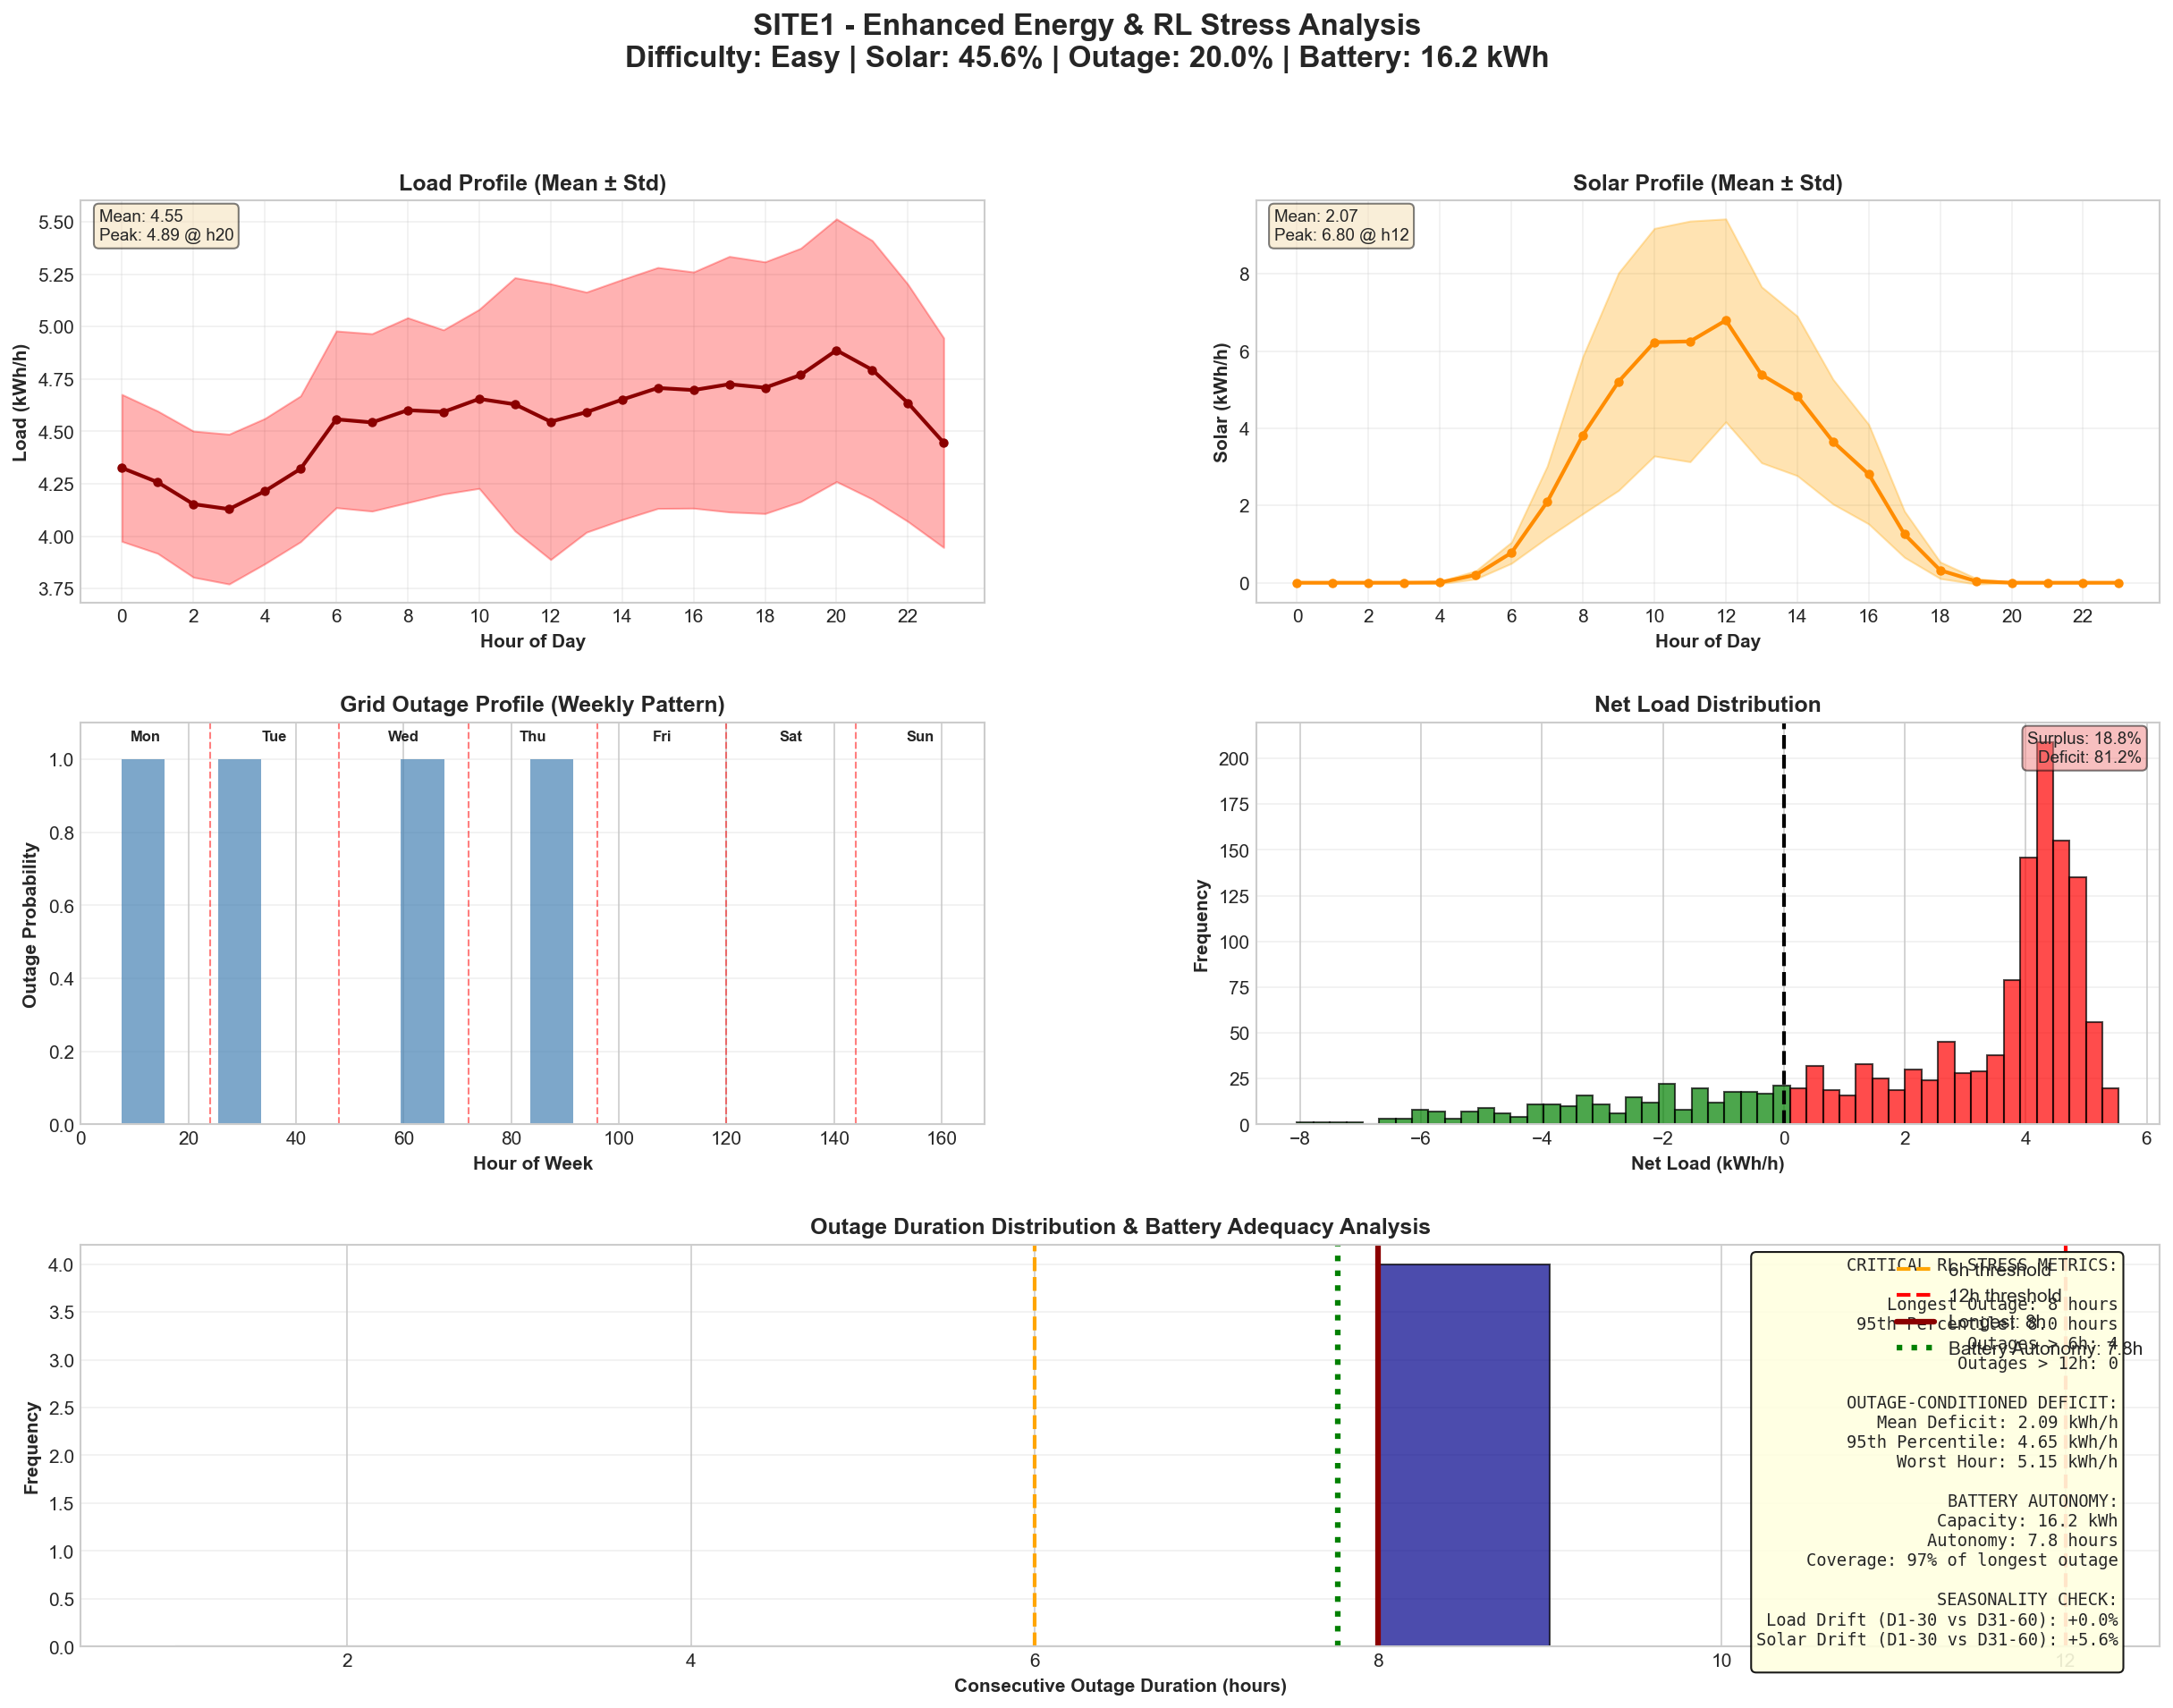
\includegraphics[width=\textwidth]{images/site1_enhanced_analysis}
\caption{Site~1 --- Easy. Load mean 4.55\,kWh/h; solar coverage 45.6\%;
grid availability 80.0\%; battery autonomy 7.8\,h (97\% of longest outage).
No outages exceed 12\,h. Outage-conditioned mean deficit 2.09\,kWh/h.}
\label{fig:app_site1}
\end{figure}

\begin{figure}[htbp]
\centering
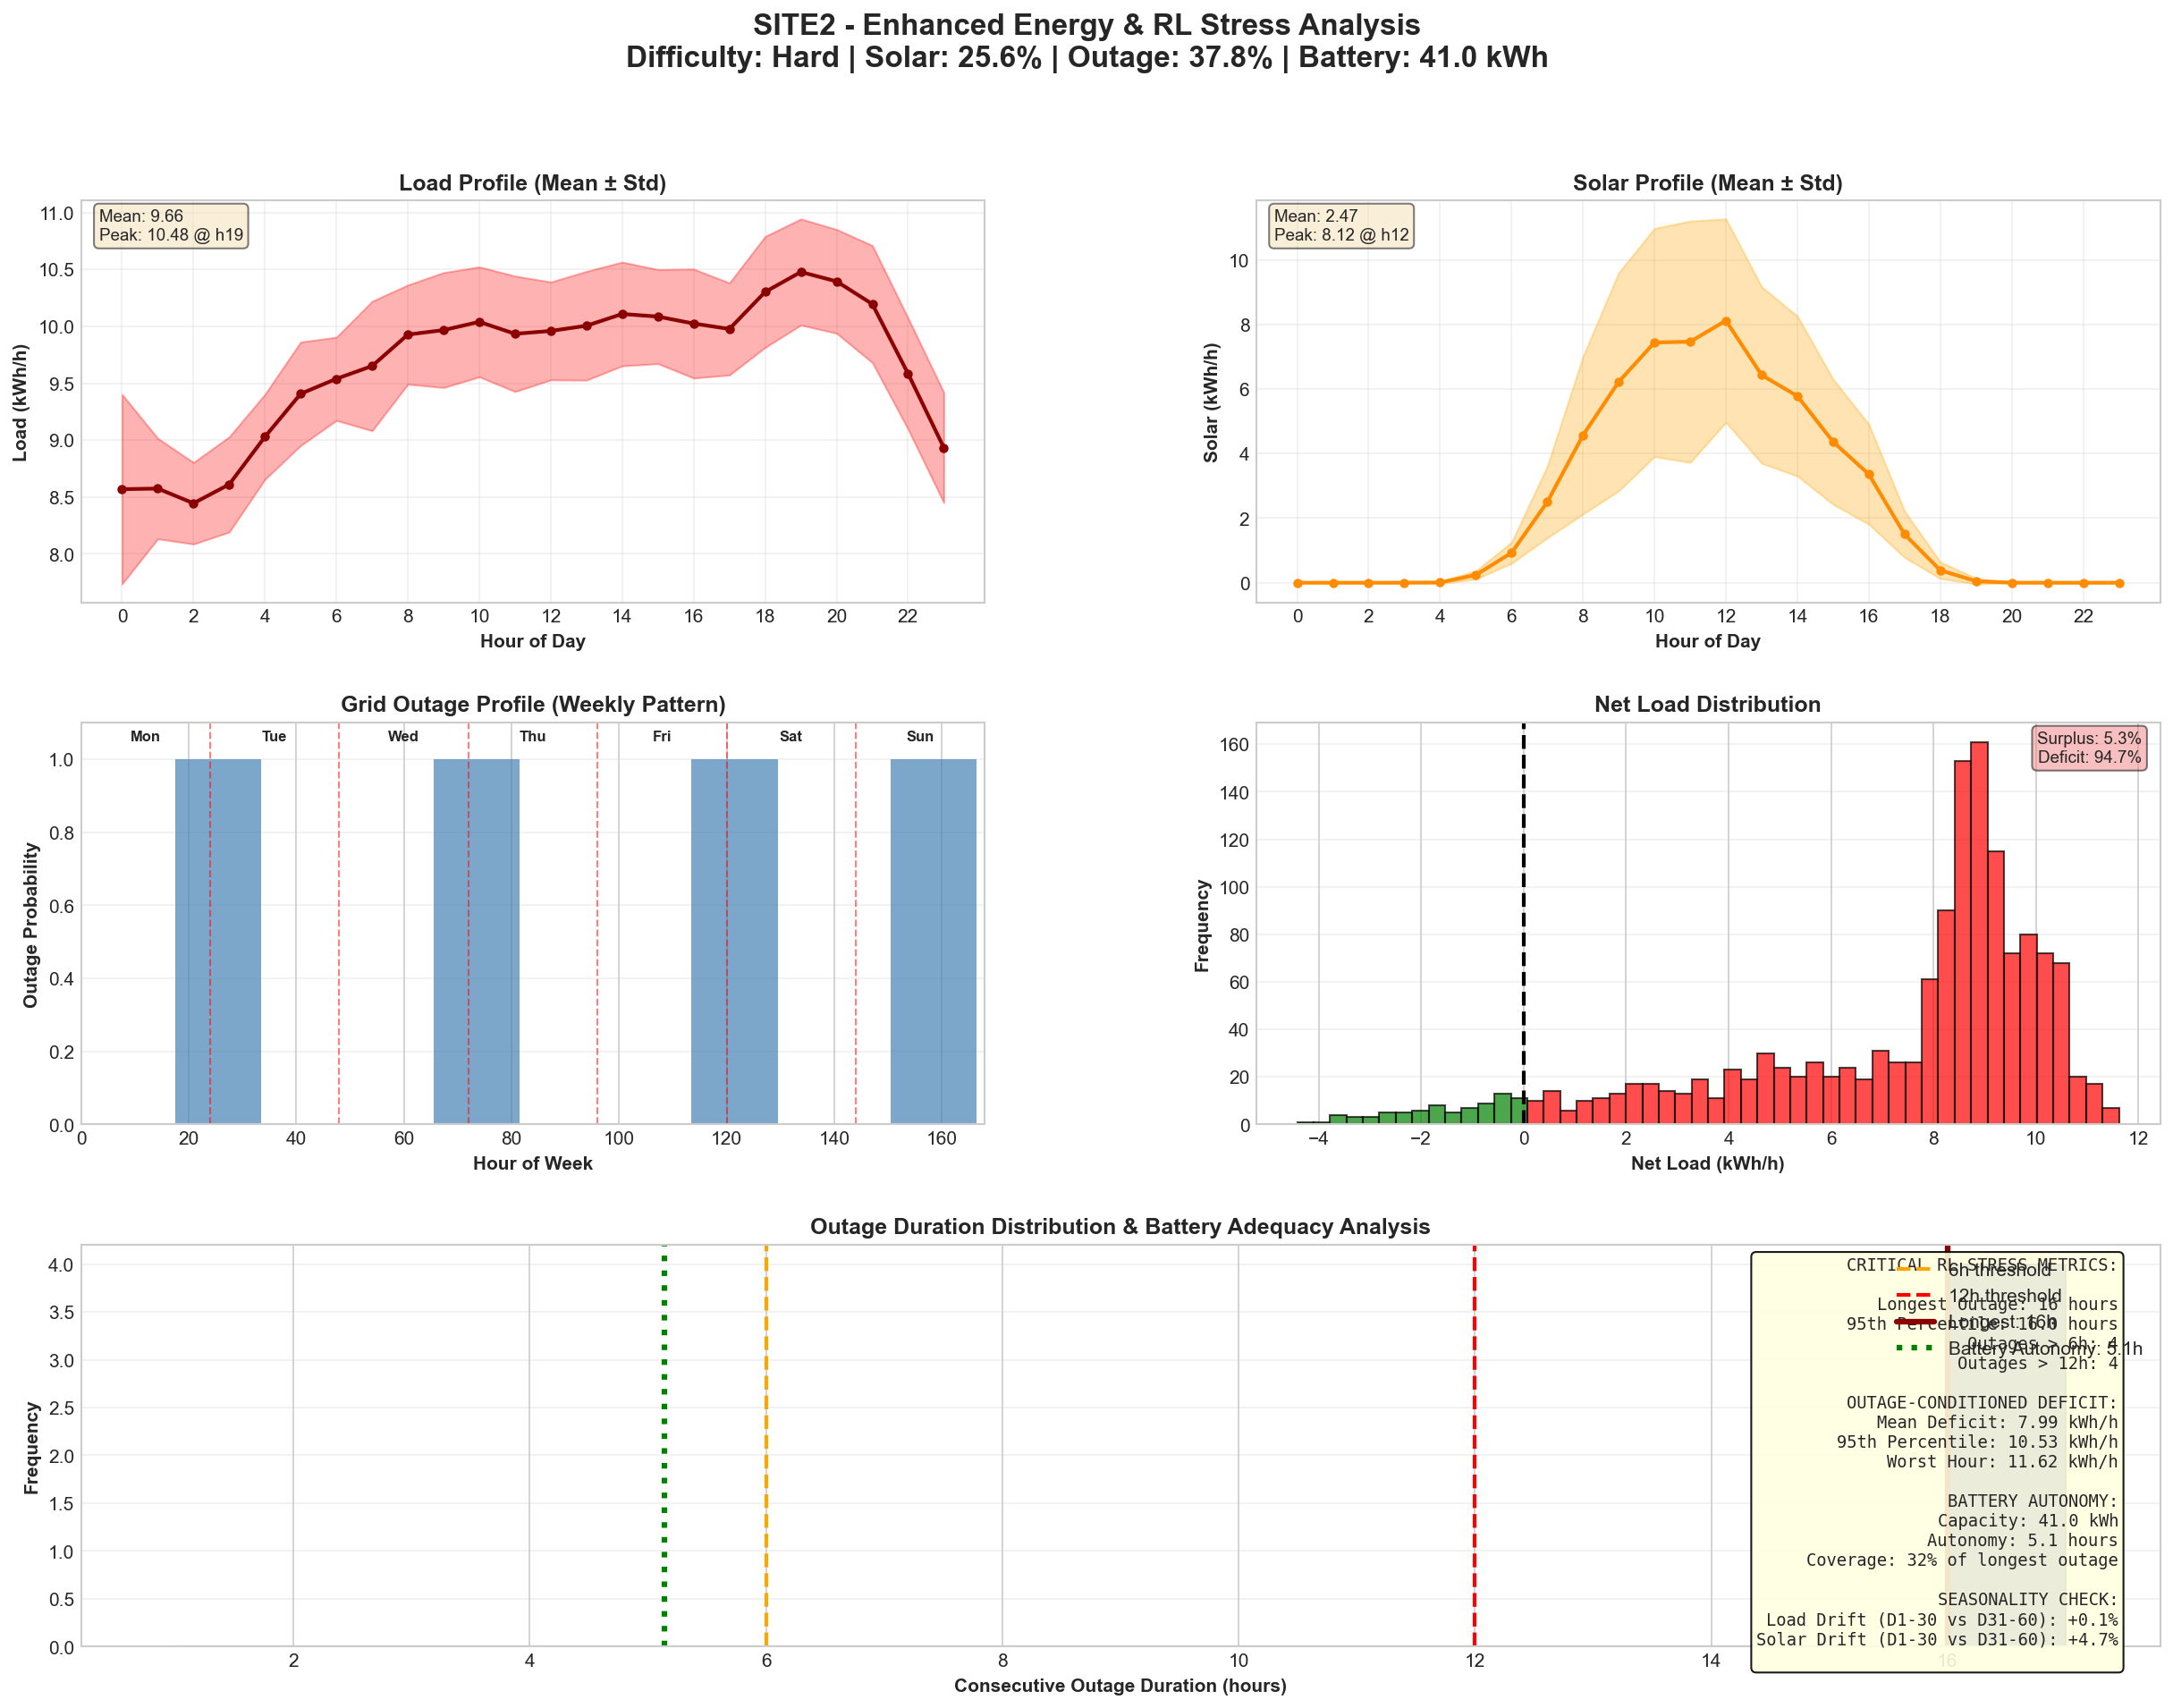
\includegraphics[width=\textwidth]{images/site2_enhanced_analysis}
\caption{Site~2 --- Hard. Load mean 9.66\,kWh/h (highest in dataset);
solar coverage 25.6\% (lowest); battery autonomy 5.1\,h (32\% of longest
outage). Four outages exceed 12\,h. Outage-conditioned mean deficit
7.99\,kWh/h.}
\label{fig:app_site2}
\end{figure}

\begin{figure}[htbp]
\centering
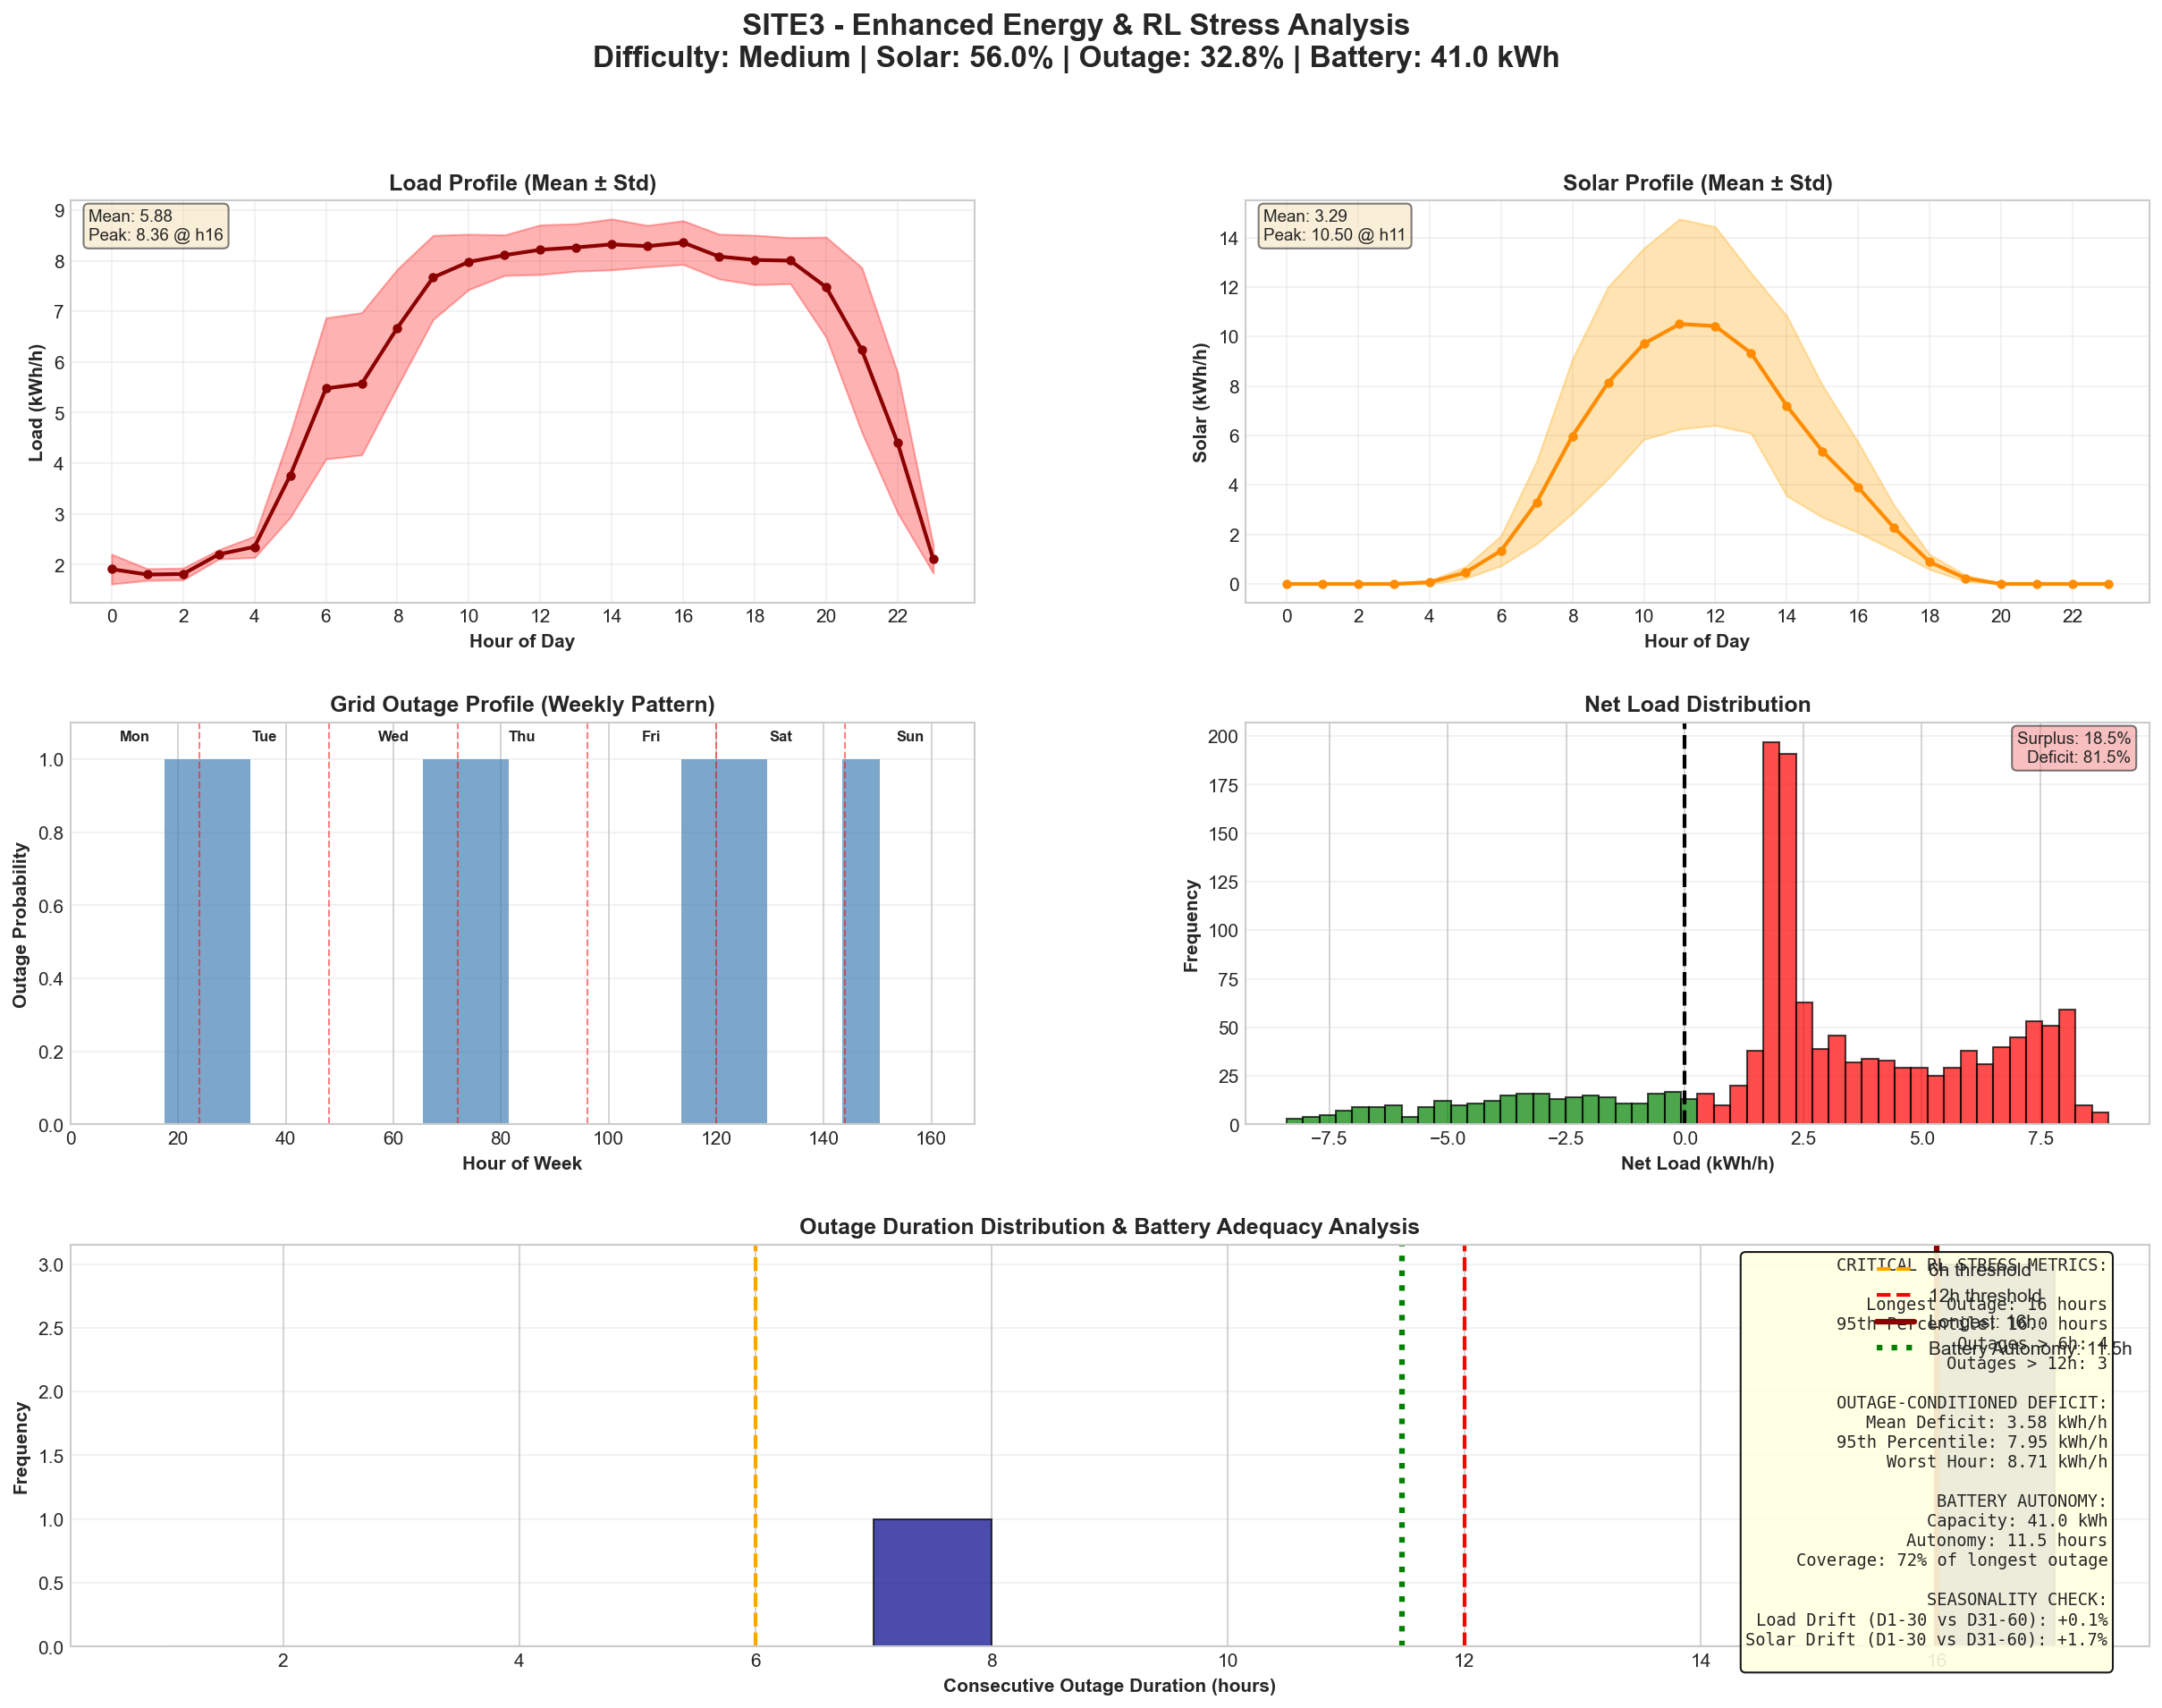
\includegraphics[width=\textwidth]{images/site3_enhanced_analysis}
\caption{Site~3 --- Medium. Load mean 5.88\,kWh/h; solar coverage 56.0\%;
battery autonomy 11.5\,h (72\% of longest outage). Three outages exceed
12\,h. Outage-conditioned mean deficit 3.58\,kWh/h.}
\label{fig:app_site3}
\end{figure}

\begin{figure}[htbp]
\centering
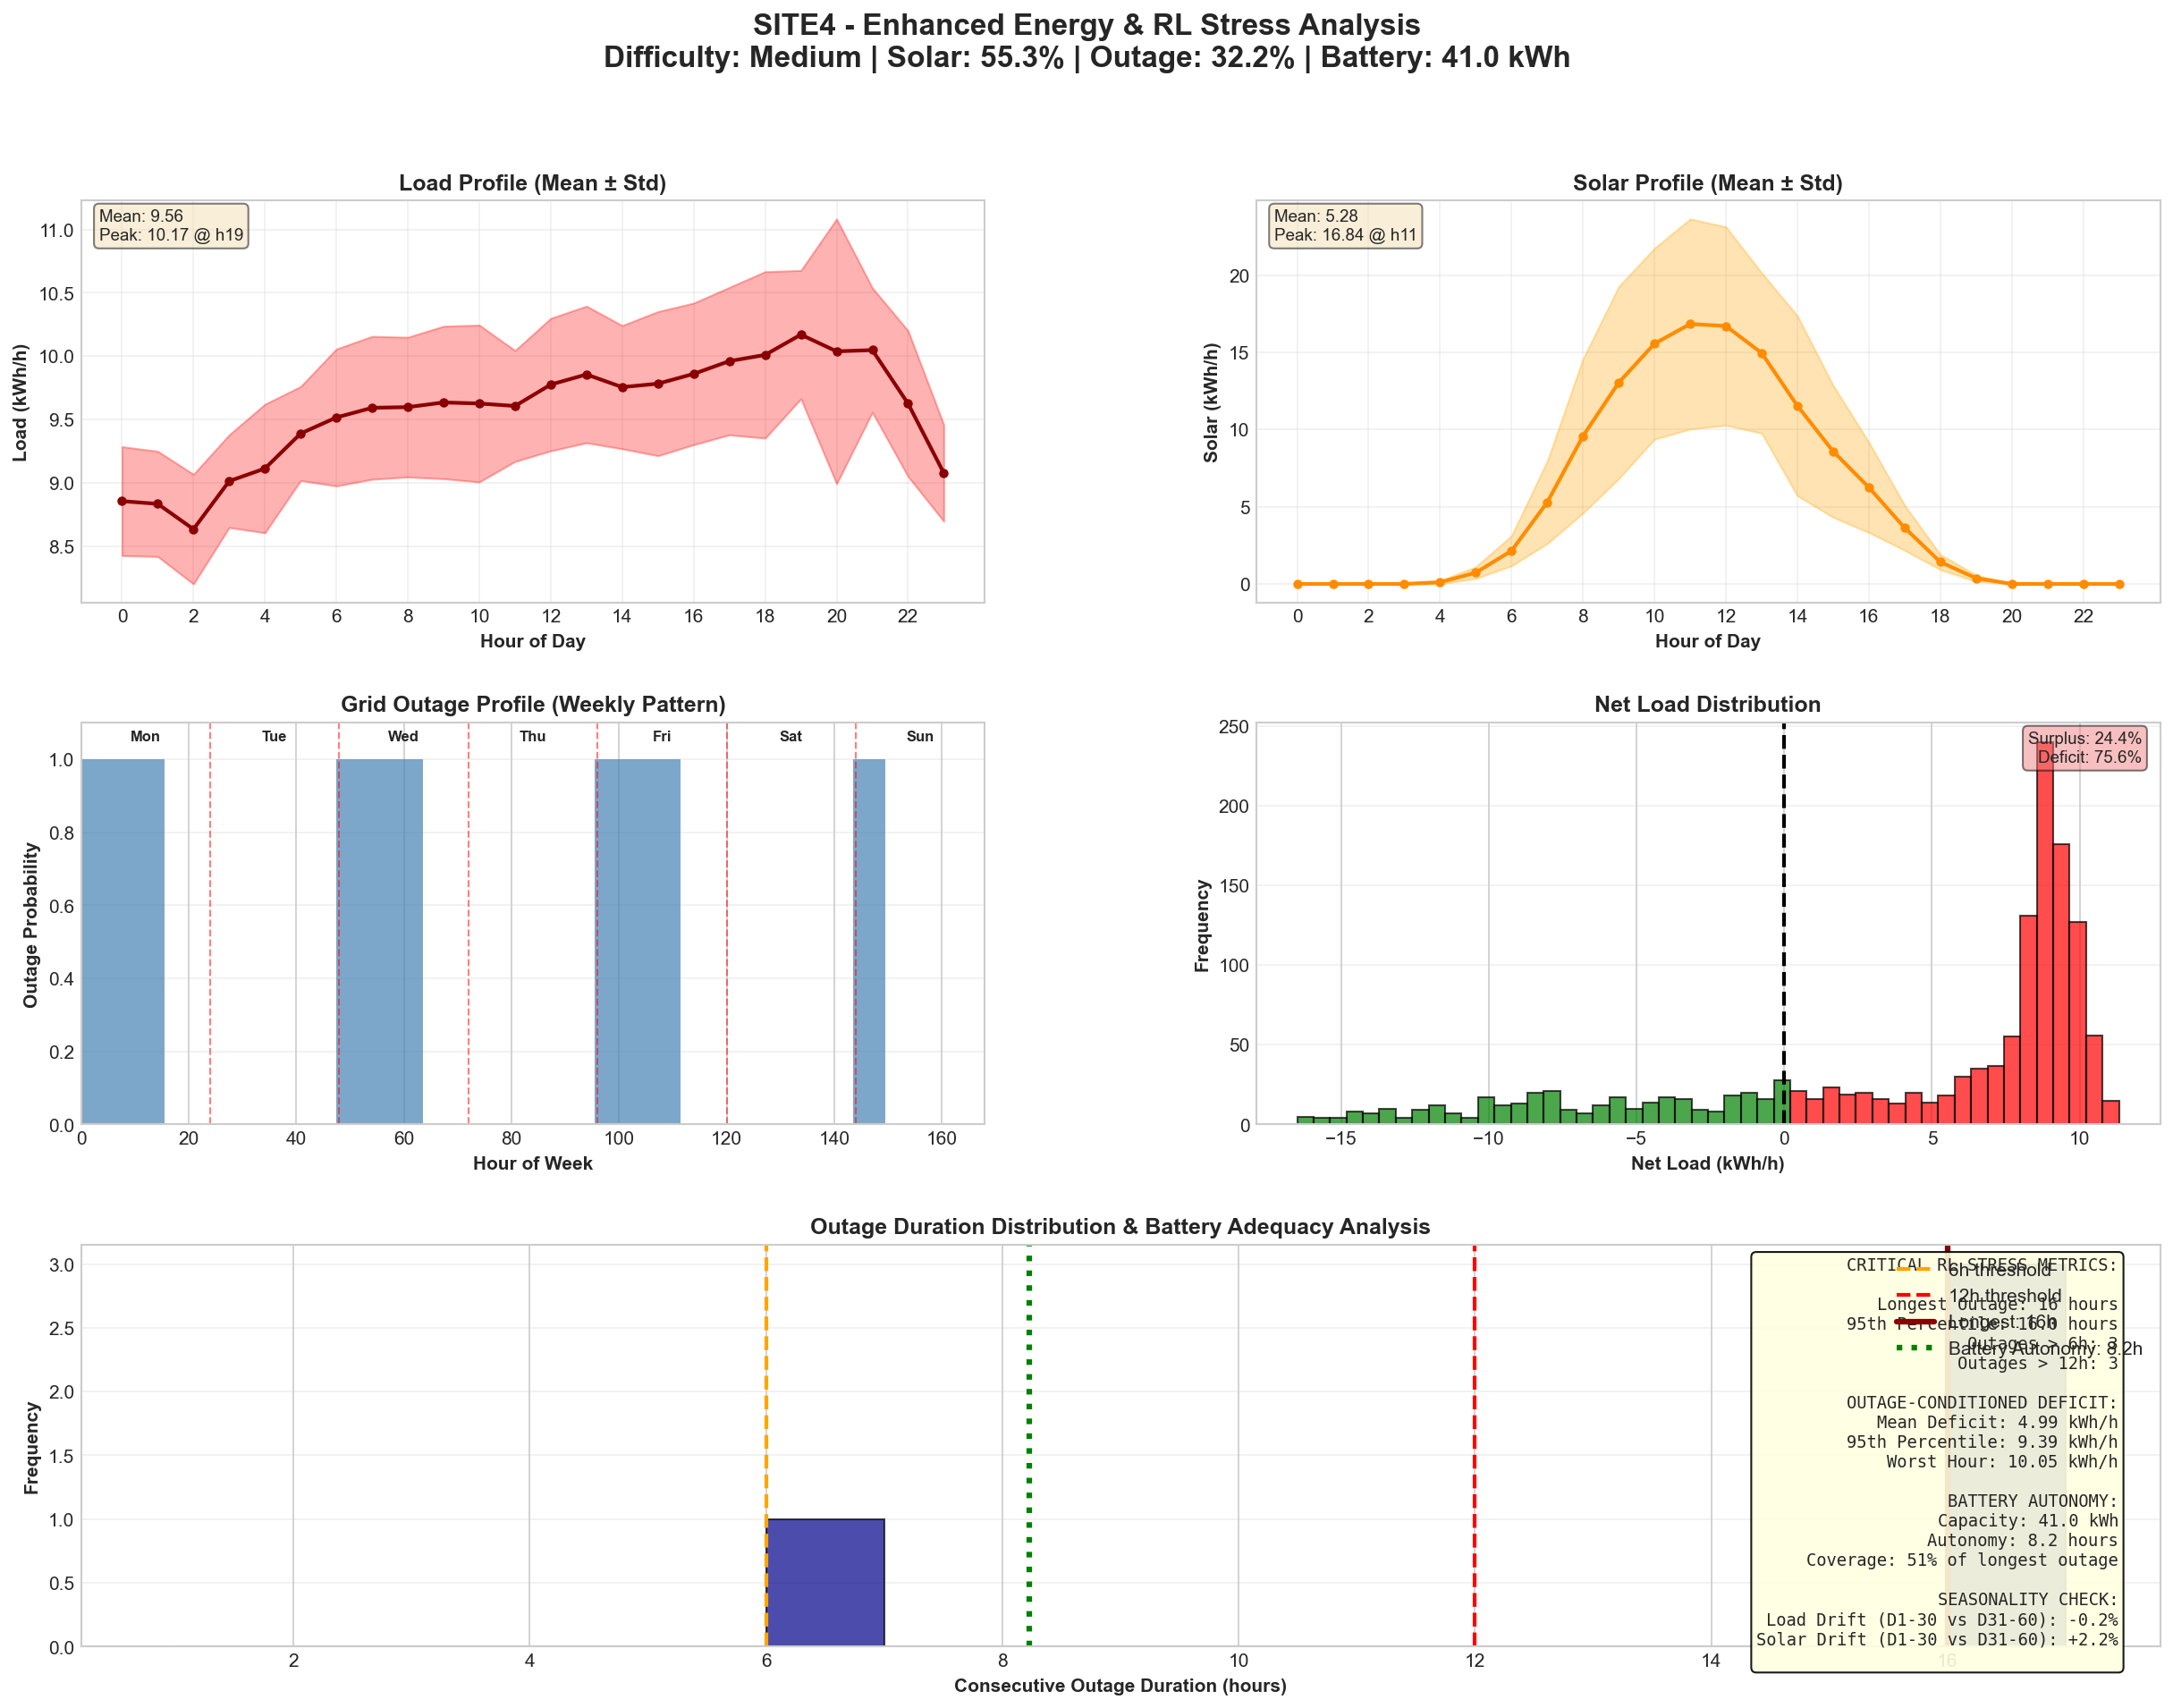
\includegraphics[width=\textwidth]{images/site4_enhanced_analysis}
\caption{Site~4 --- Medium. Load mean 9.56\,kWh/h; solar coverage 55.3\%;
battery autonomy 8.2\,h (51\% of longest outage). Three outages exceed
12\,h. Outage-conditioned mean deficit 4.99\,kWh/h. Notable for
combining high load with reasonable solar coverage.}
\label{fig:app_site4}
\end{figure}

\begin{figure}[htbp]
\centering
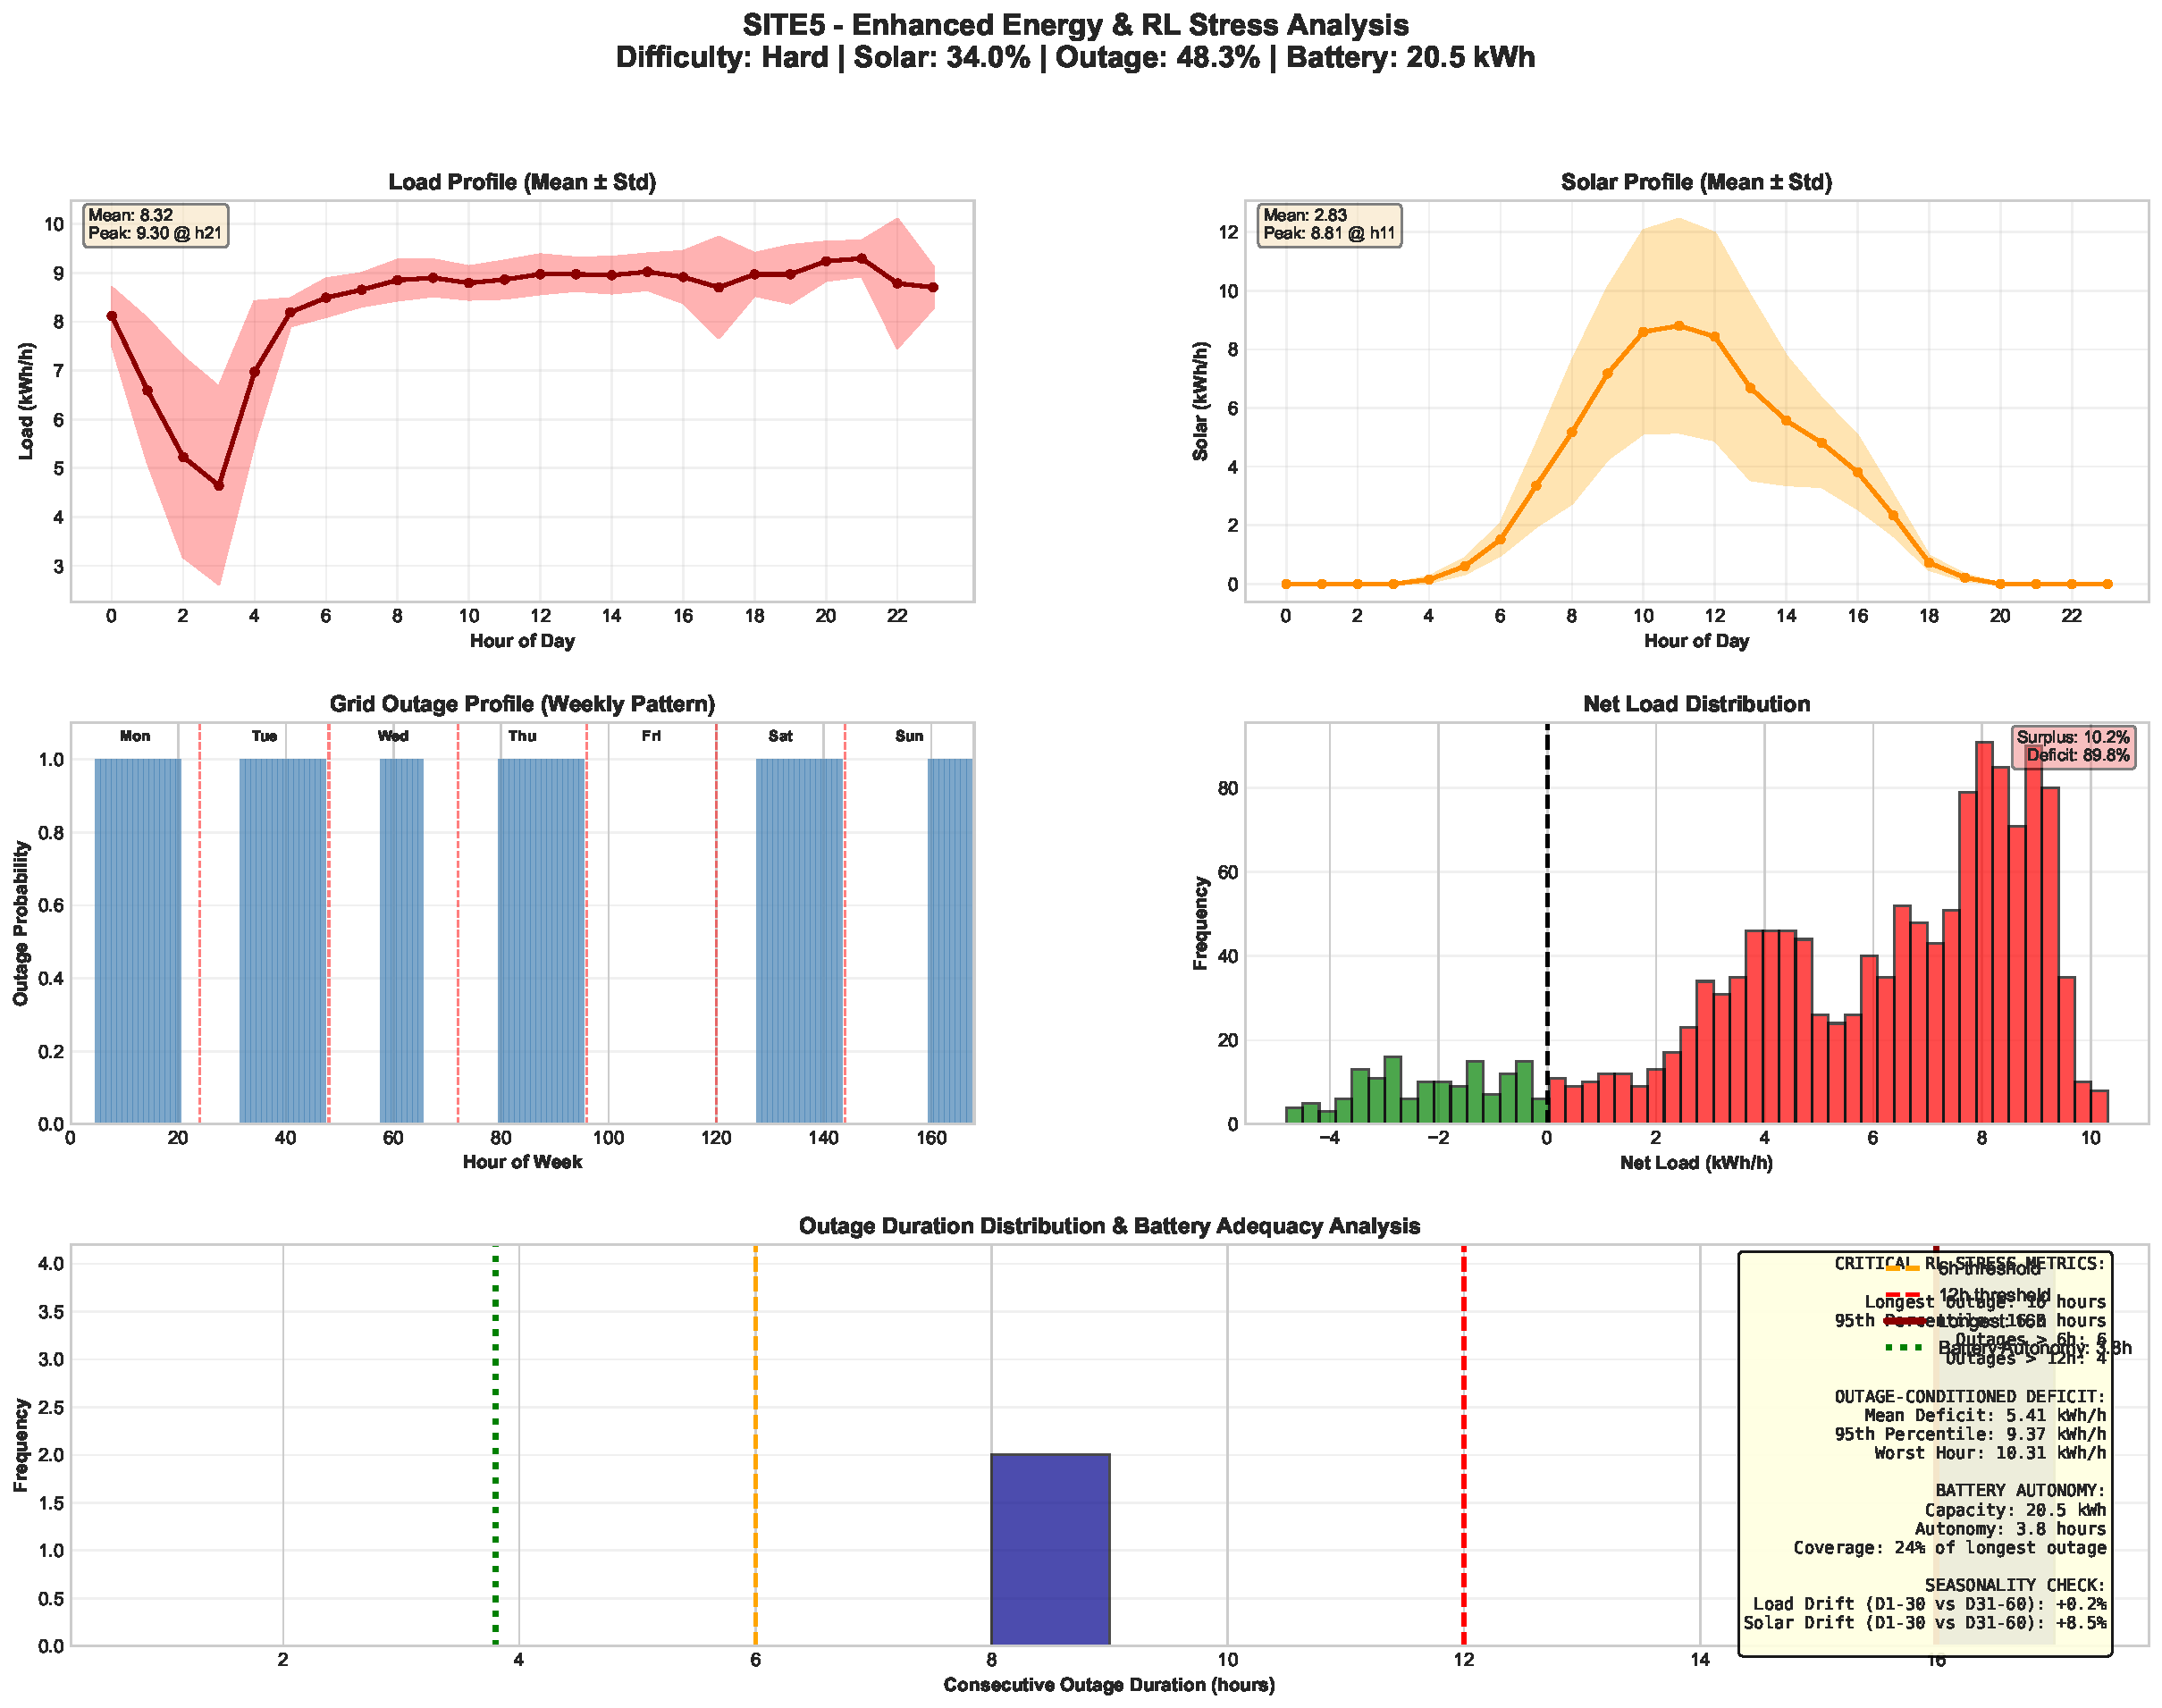
\includegraphics[width=\textwidth]{images/site5_enhanced_analysis}
\caption{Site~5 --- Hard. Load mean 8.32\,kWh/h; solar coverage 34.0\%;
battery autonomy 3.8\,h (24\% of longest outage). 52 outage events ---
highest frequency in dataset. Four outages exceed 12\,h.
Outage-conditioned mean deficit 5.41\,kWh/h.}
\label{fig:app_site5}
\end{figure}

\begin{figure}[htbp]
\centering
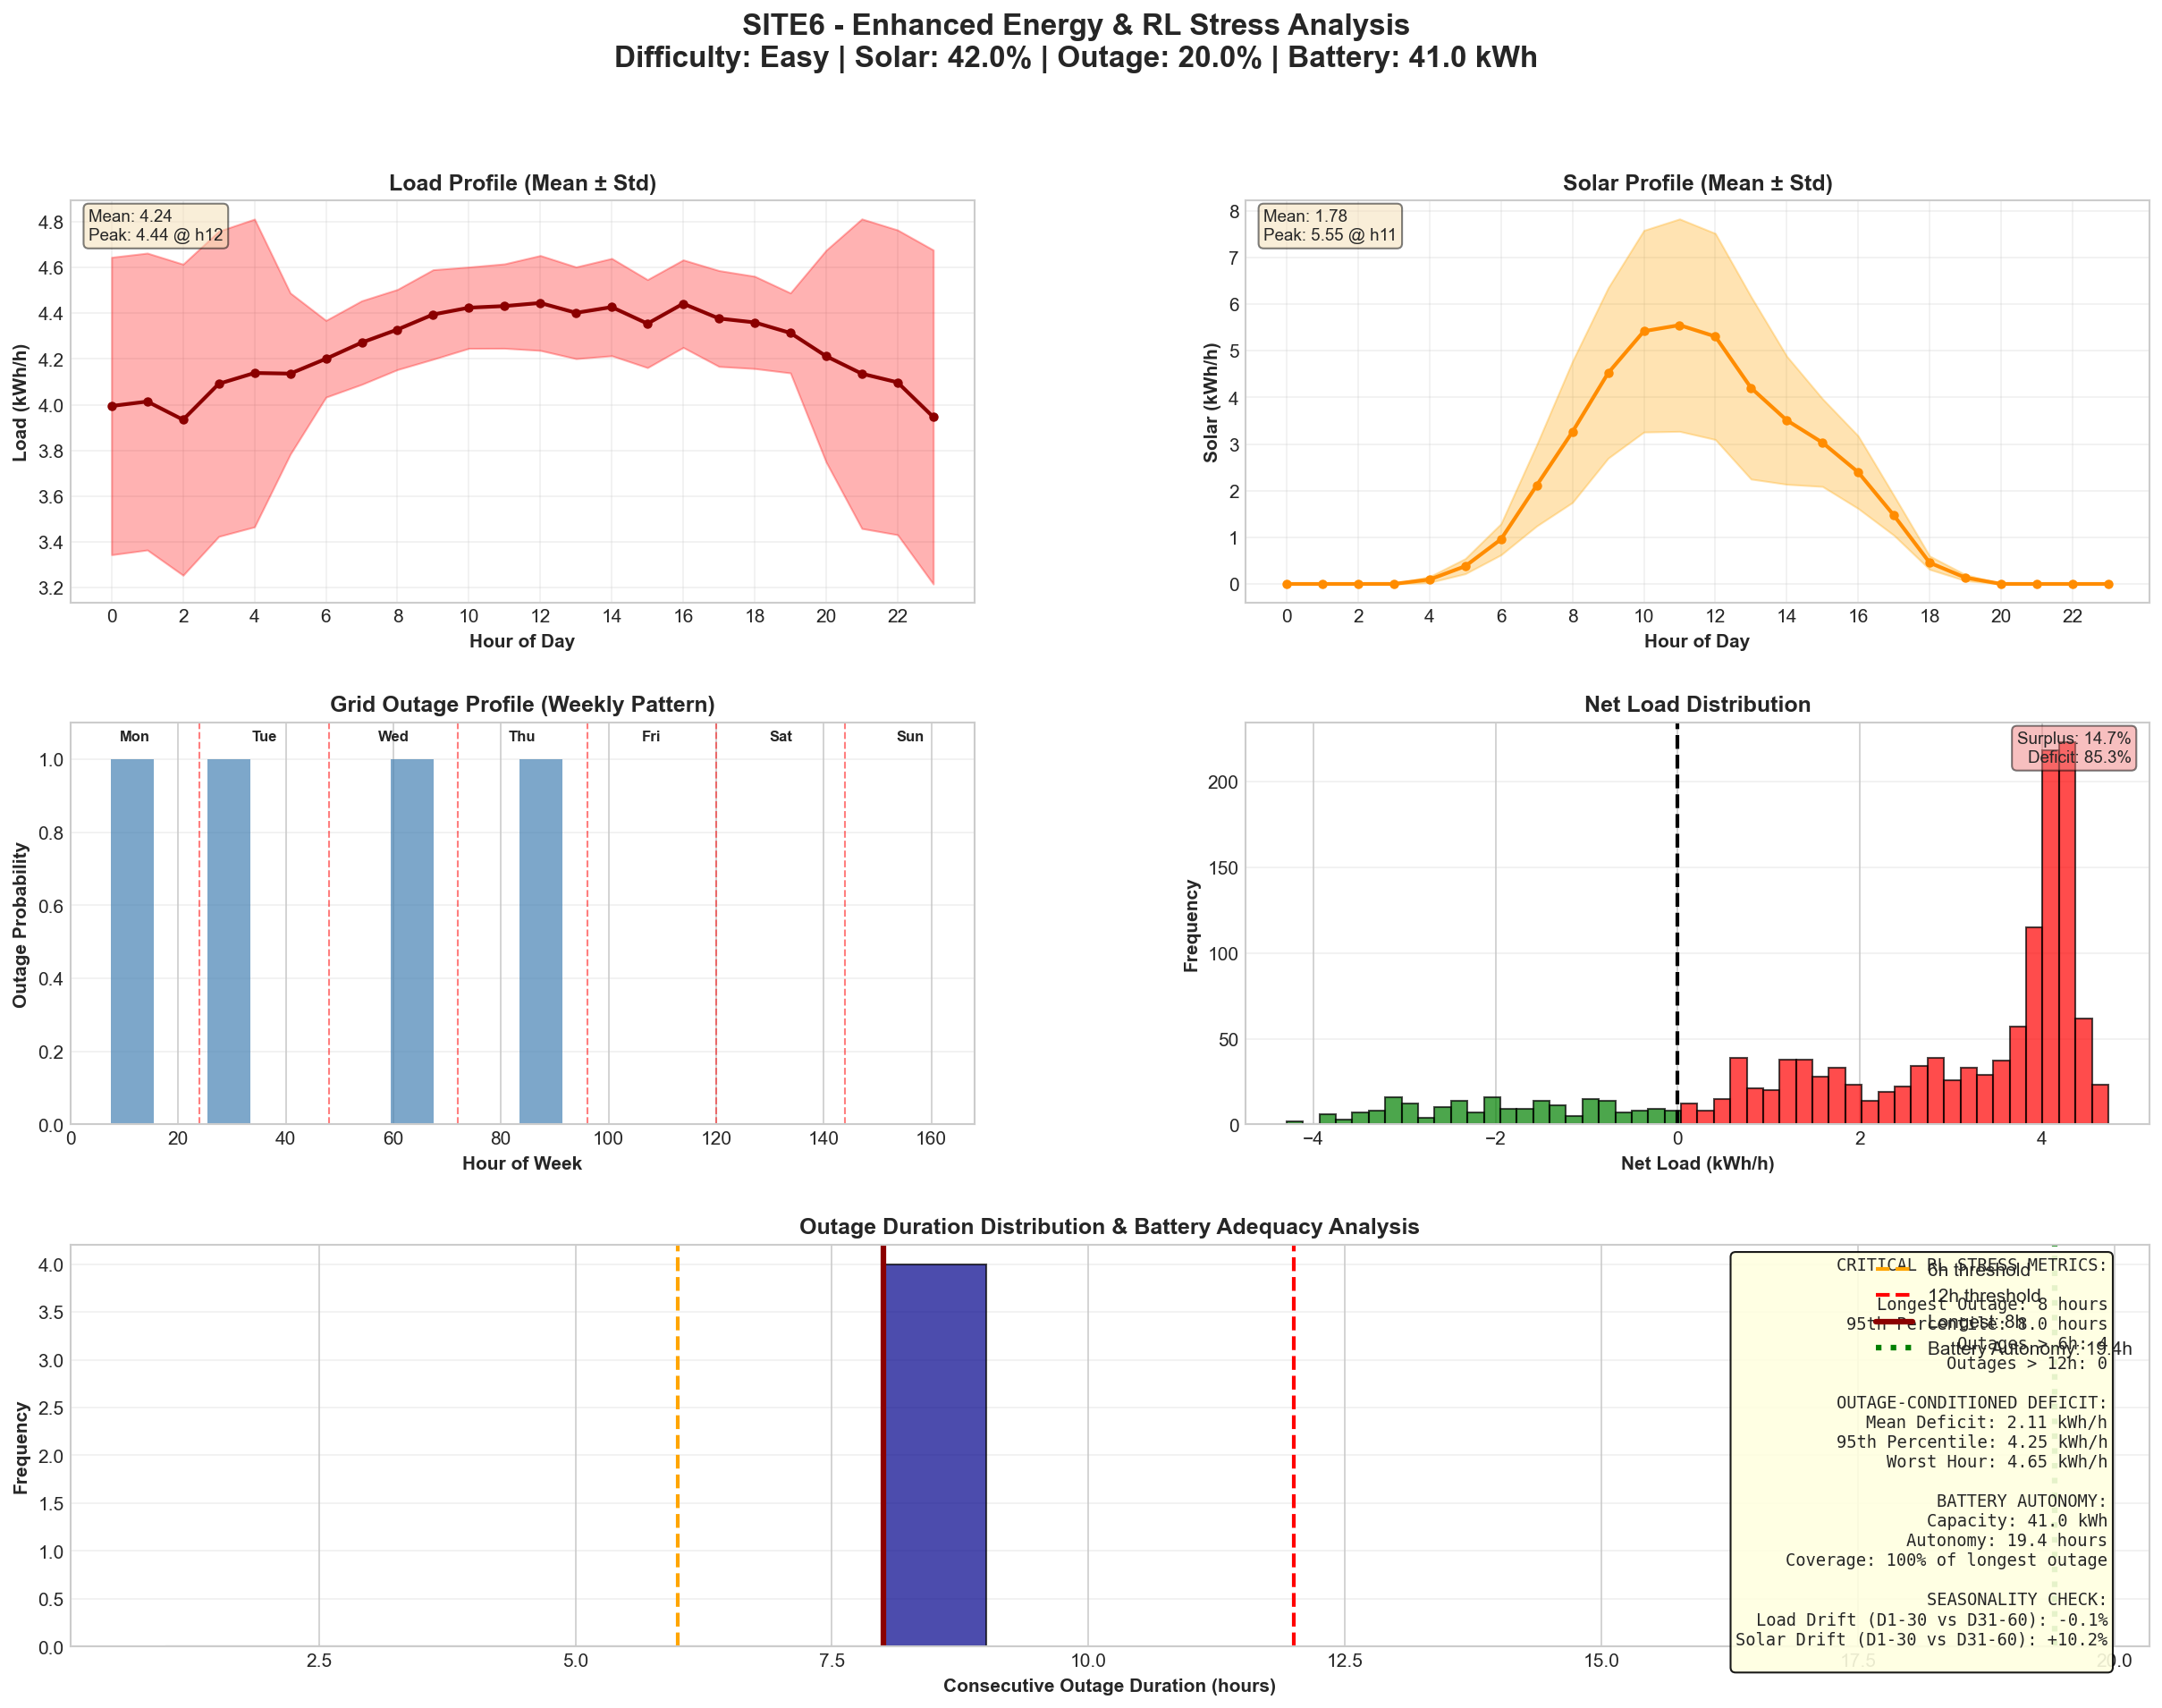
\includegraphics[width=\textwidth]{images/site6_enhanced_analysis}
\caption{Site~6 --- Easy. Load mean 4.24\,kWh/h; solar coverage 42.0\%;
grid availability 80.0\%; battery autonomy 19.4\,h (100\% of longest
outage). No outages exceed 12\,h. Outage-conditioned mean deficit
2.11\,kWh/h. Site~6 is the most battery-adequate site in the dataset.}
\label{fig:app_site6}
\end{figure}

\begin{figure}[htbp]
\centering
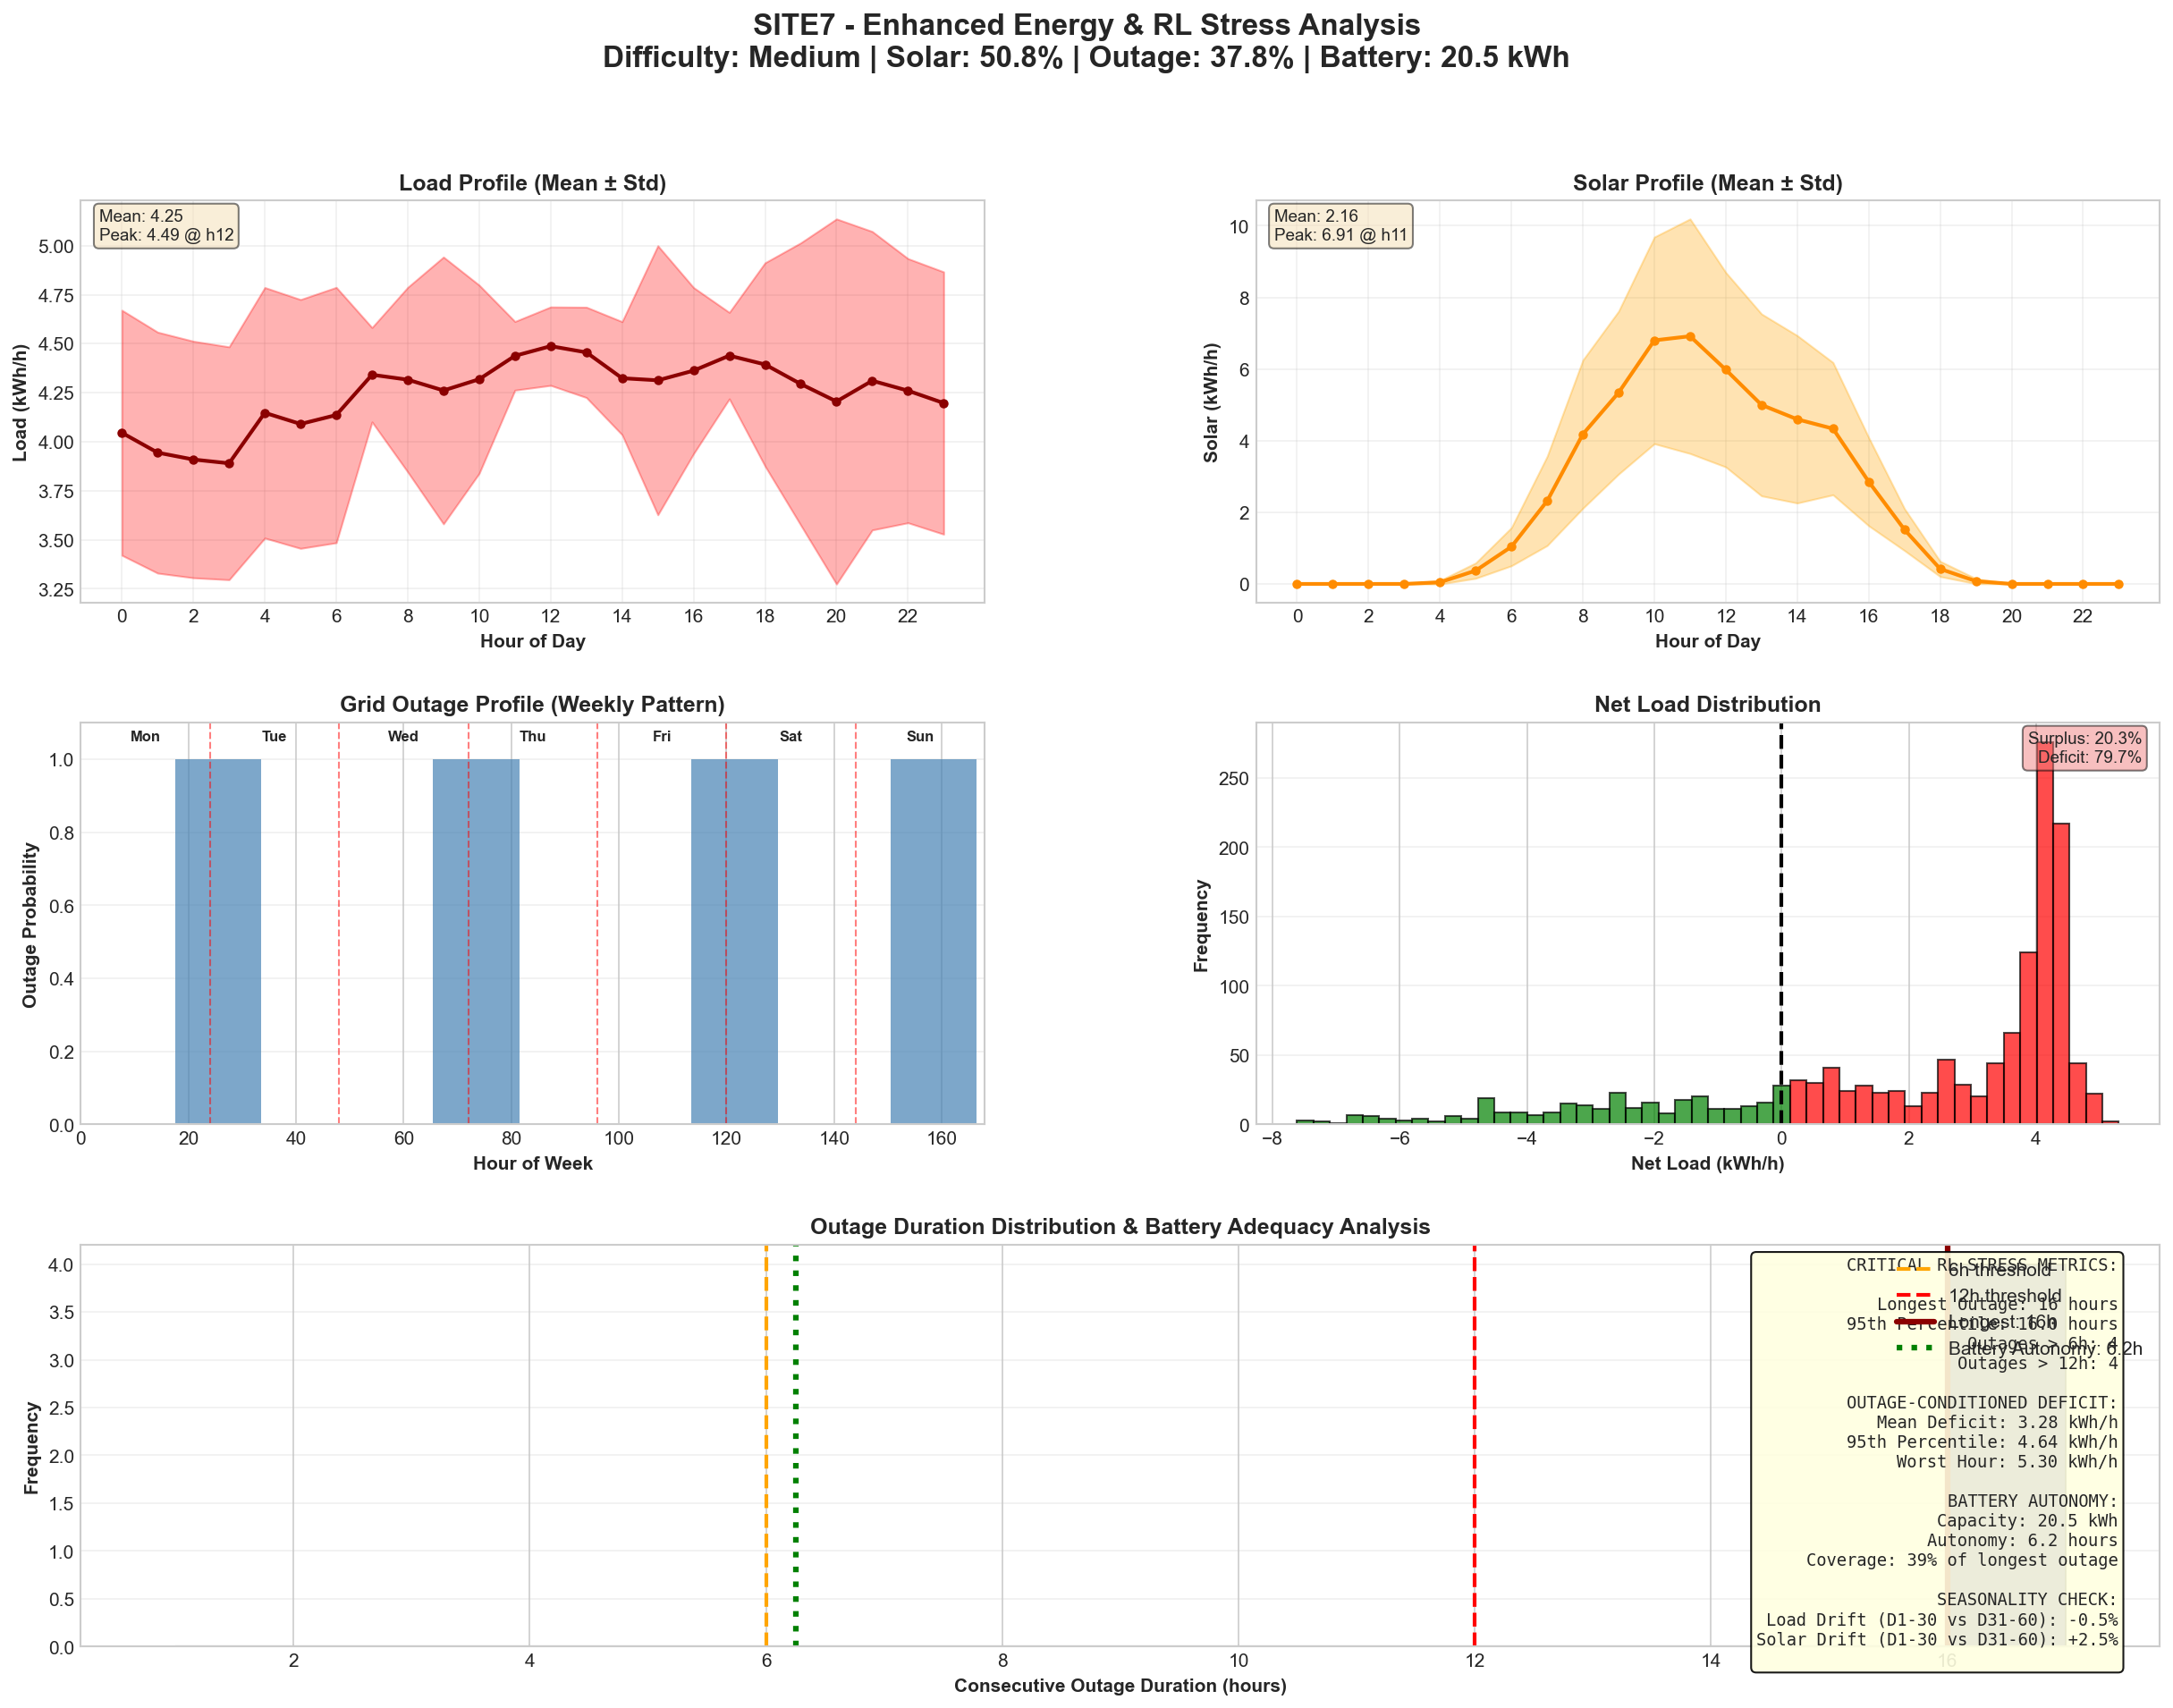
\includegraphics[width=\textwidth]{images/site7_enhanced_analysis}
\caption{Site~7 --- Medium. Load mean 4.25\,kWh/h; solar coverage 50.8\%;
battery autonomy 6.2\,h (39\% of longest outage). Four outages exceed
12\,h. Outage-conditioned mean deficit 3.28\,kWh/h. Despite moderate
load, battery undersizing relative to 16-hour outages creates reliability
risk.}
\label{fig:app_site7}
\end{figure}

\begin{figure}[htbp]
\centering
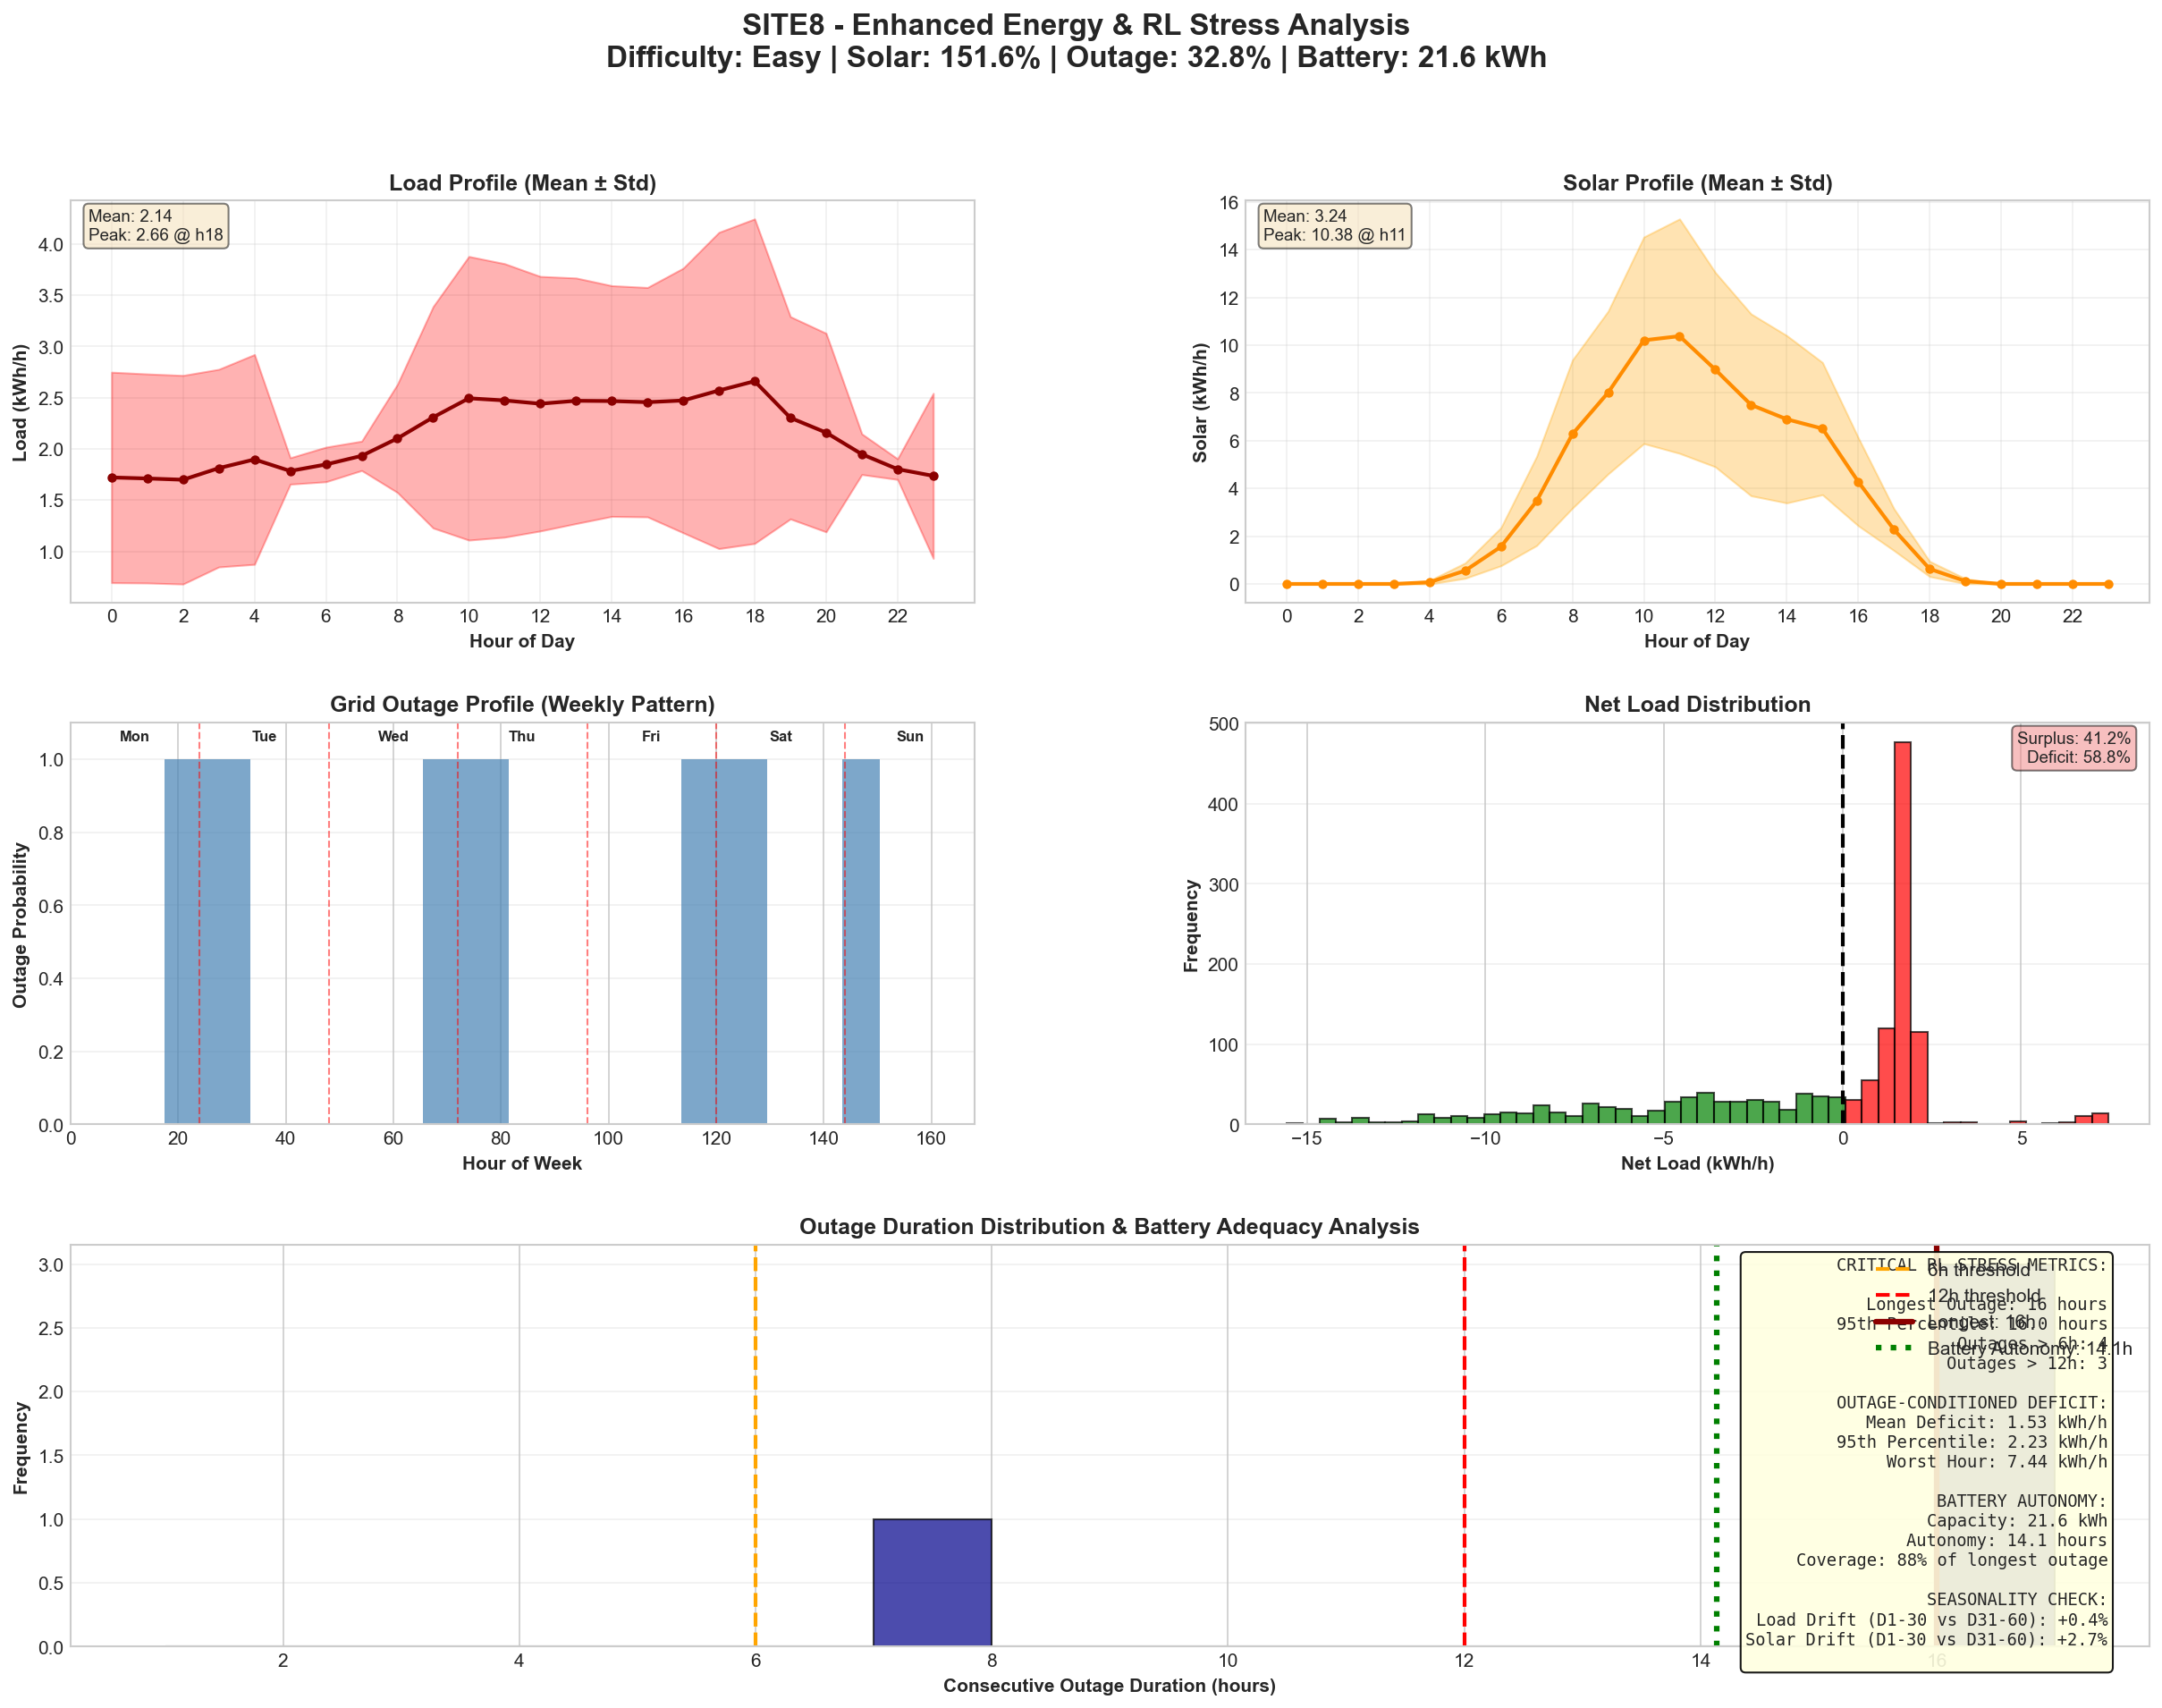
\includegraphics[width=\textwidth]{images/site8_enhanced_analysis}
\caption{Site~8 --- Easy (solar surplus). Load mean 2.14\,kWh/h; solar
coverage 151.6\%; battery autonomy 14.1\,h (88\% of longest outage).
41.2\% of hours are solar-surplus. Three outages exceed 12\,h but
outage-conditioned mean deficit is only 1.53\,kWh/h. Primary challenge
is battery saturation and curtailment, not stockout.}
\label{fig:app_site8}
\end{figure}

\begin{figure}[htbp]
\centering
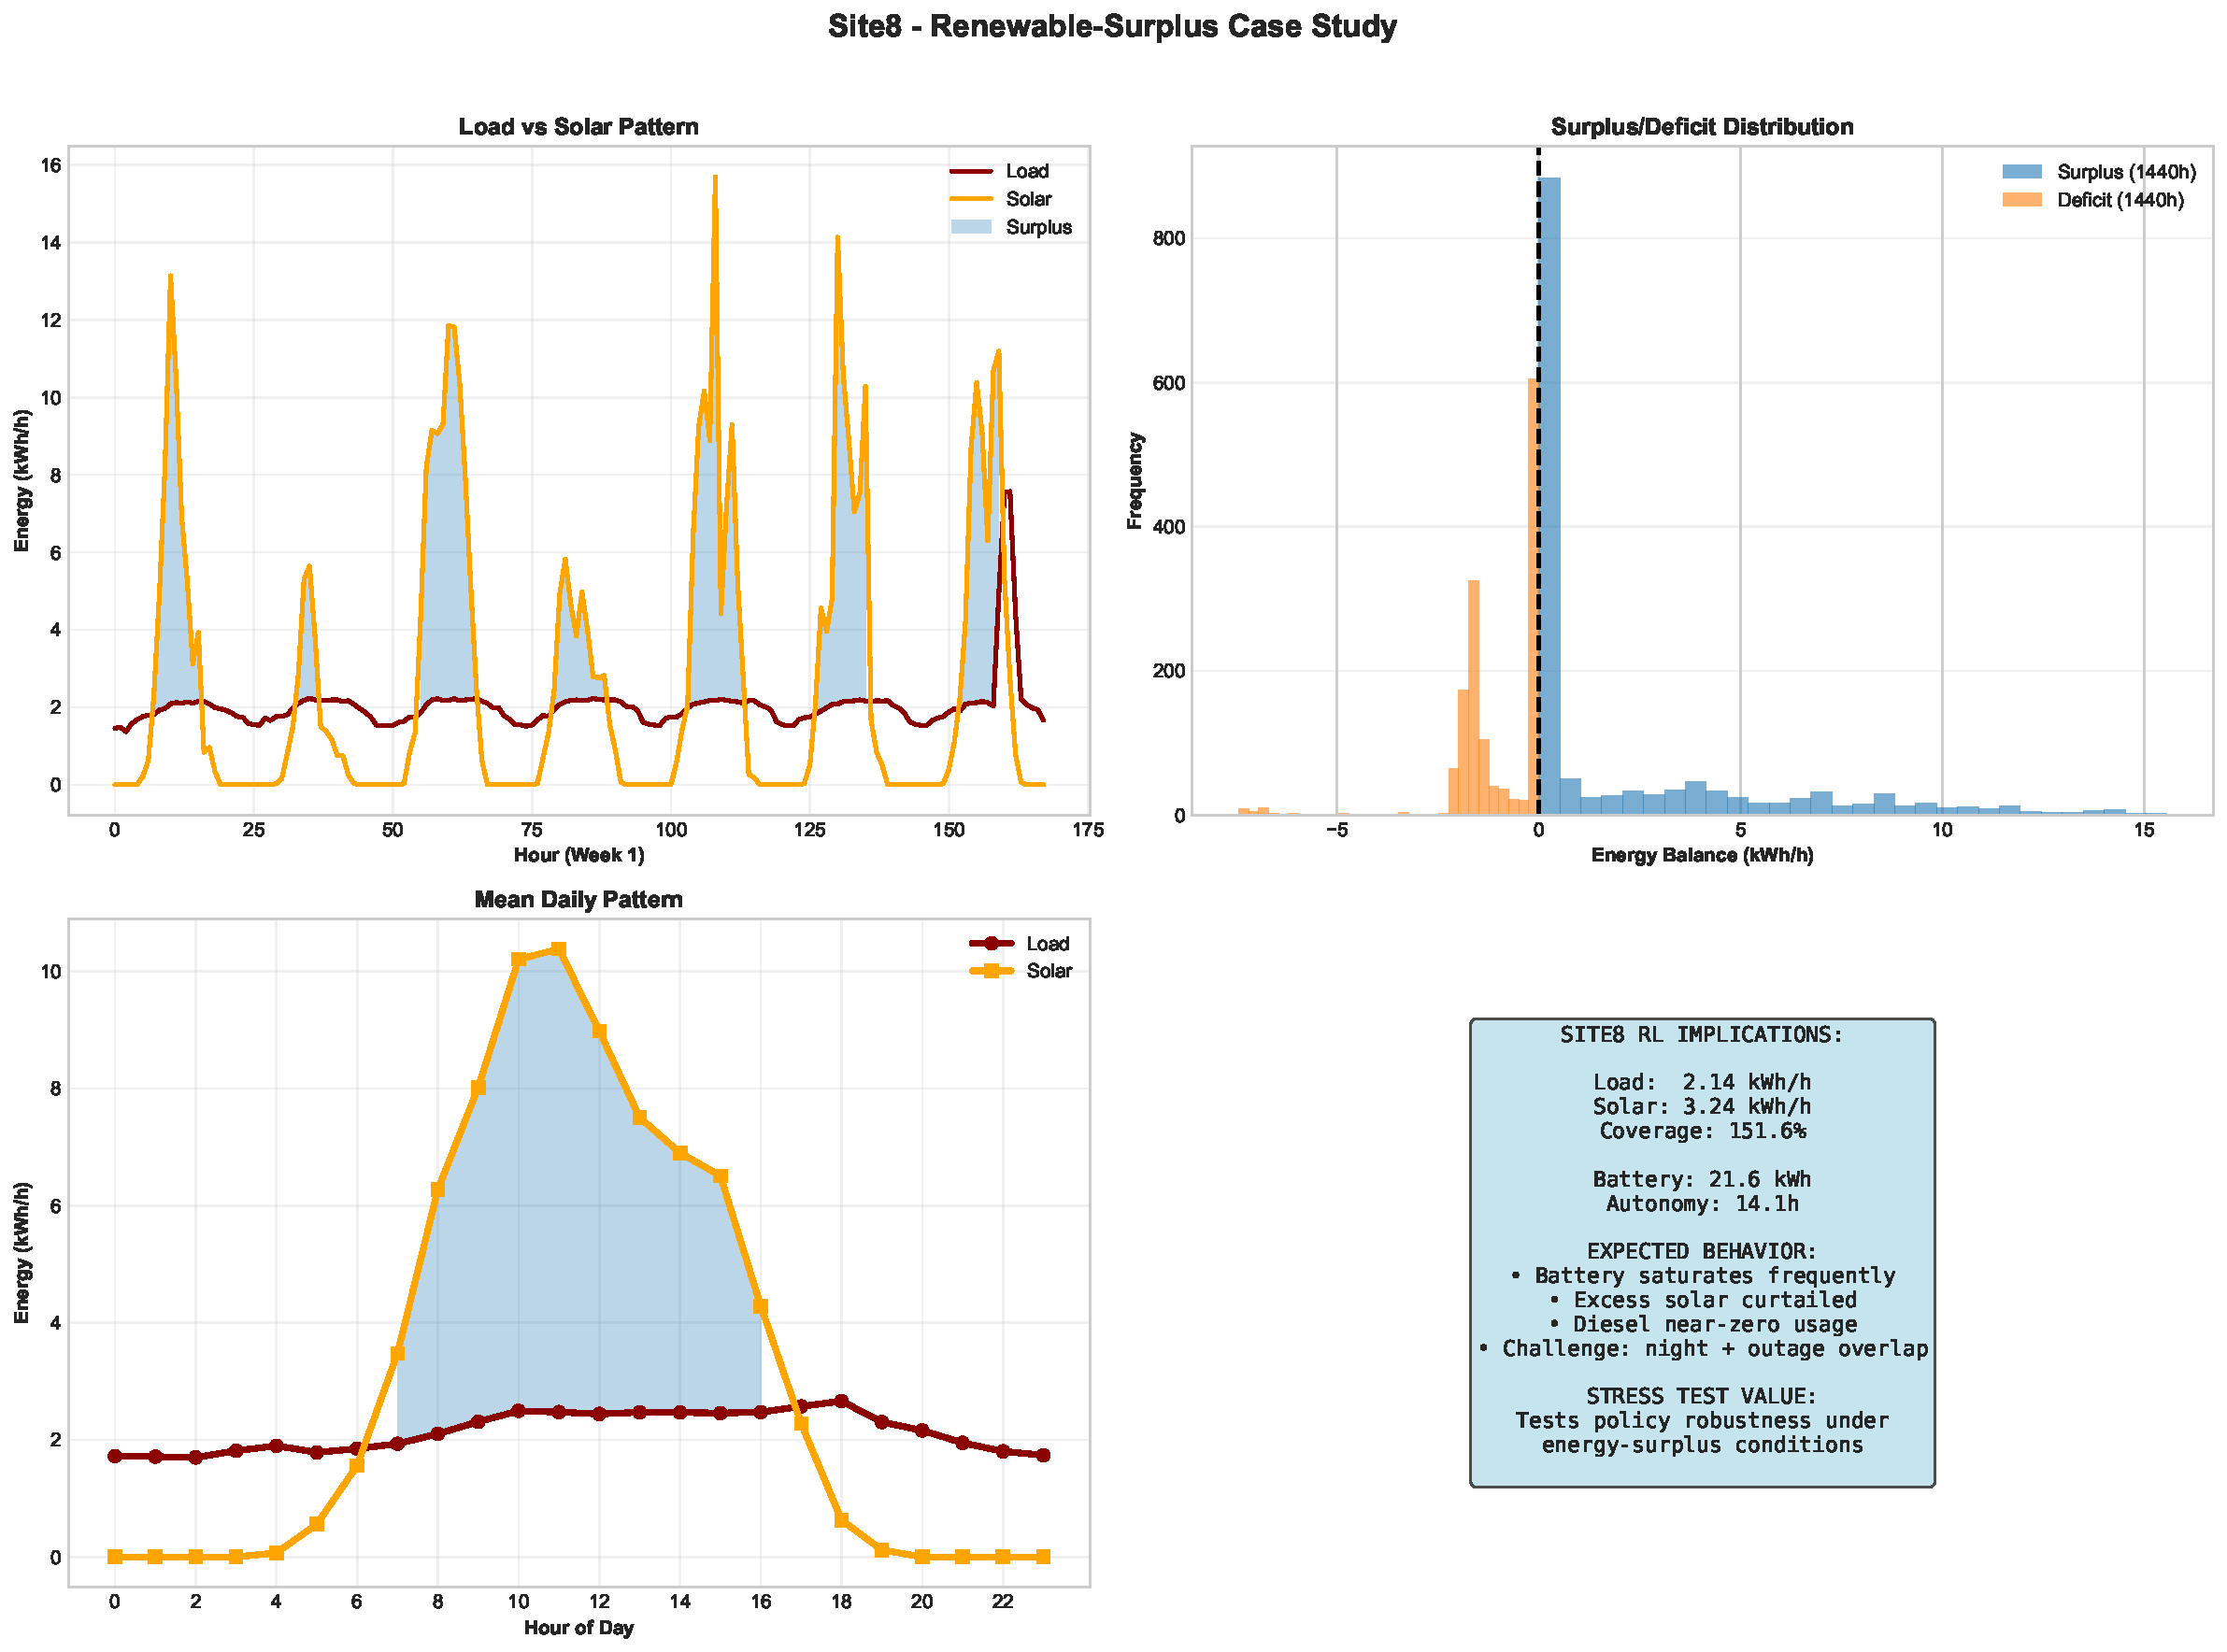
\includegraphics[width=\textwidth]{images/fig3_site8_surplus}
\caption{Site~8 renewable-surplus case study showing load vs.\ solar time
series (top-left), surplus/deficit distribution (top-right), and mean
daily pattern (bottom-left). 41\% of hours are solar-surplus; average
surplus 51\,kWh/day.}
\label{fig:app_site8_surplus}
\end{figure}

\begin{figure}[htbp]
\centering
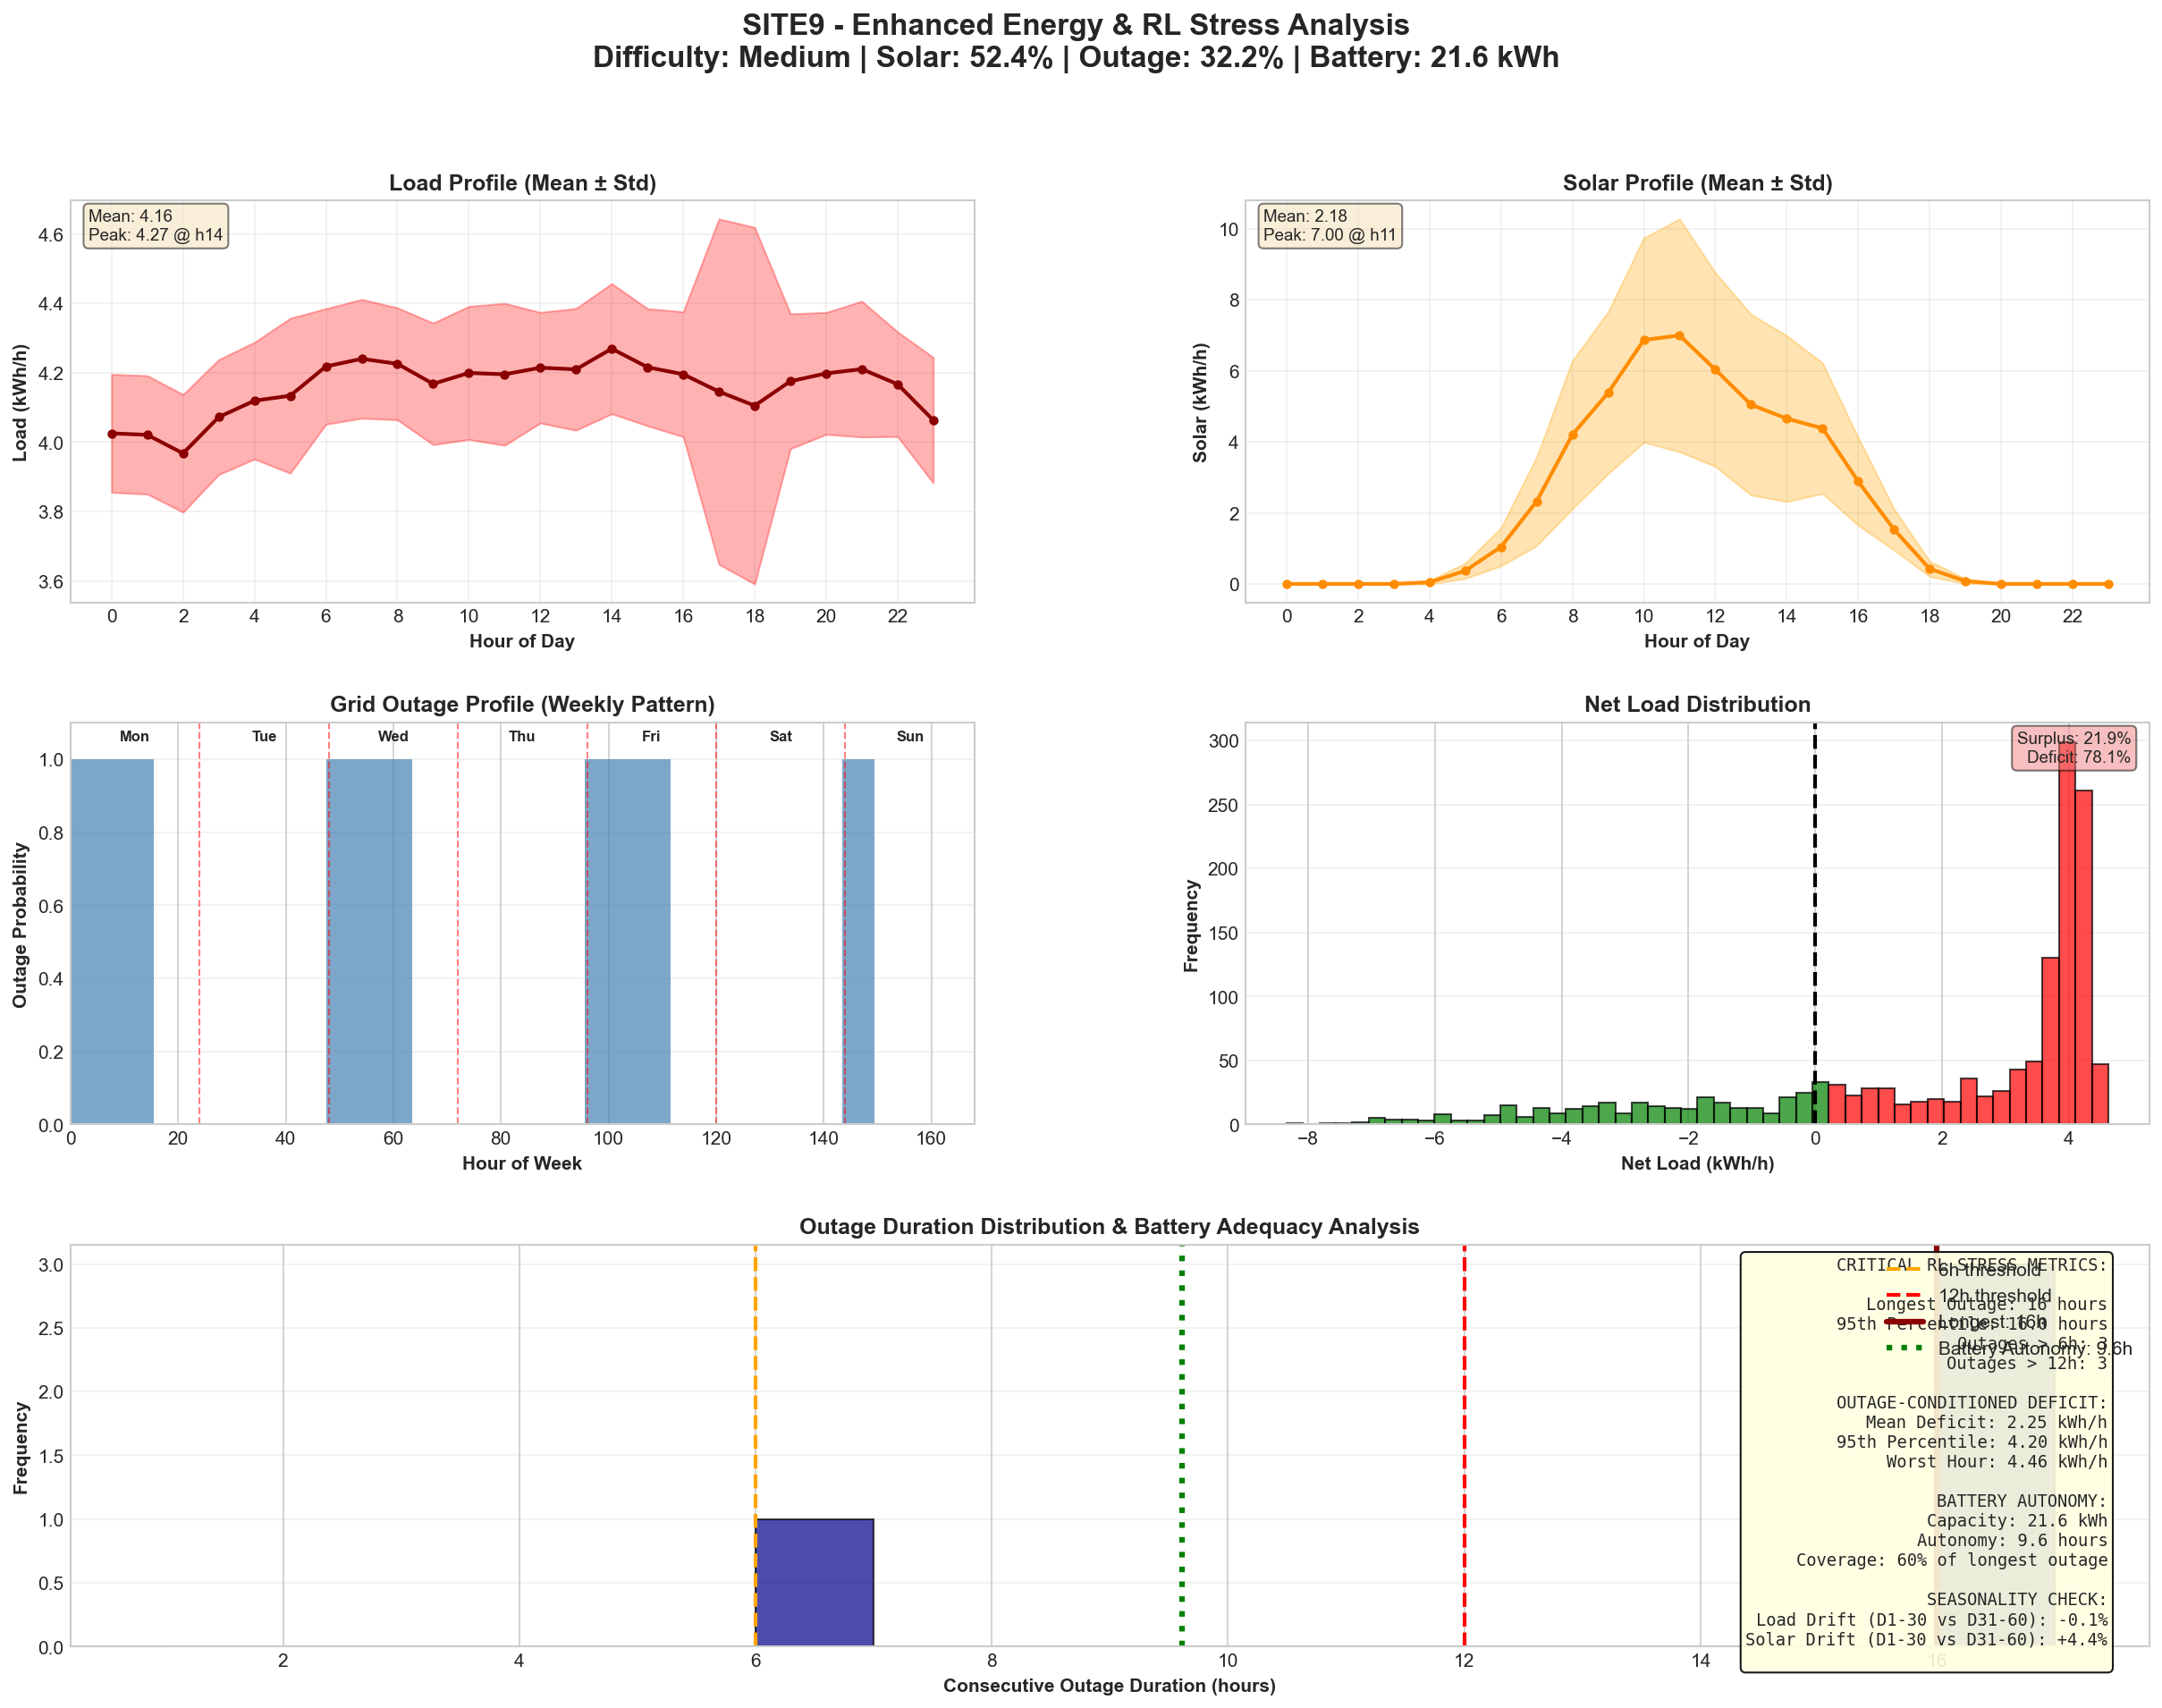
\includegraphics[width=\textwidth]{images/site9_enhanced_analysis}
\caption{Site~9 --- Medium. Load mean 4.16\,kWh/h; solar coverage 52.4\%;
battery autonomy 9.6\,h (60\% of longest outage). Three outages exceed
12\,h. Outage-conditioned mean deficit 2.25\,kWh/h. Moderate difficulty
across all dimensions.}
\label{fig:app_site9}
\end{figure}

\begin{figure}[htbp]
\centering
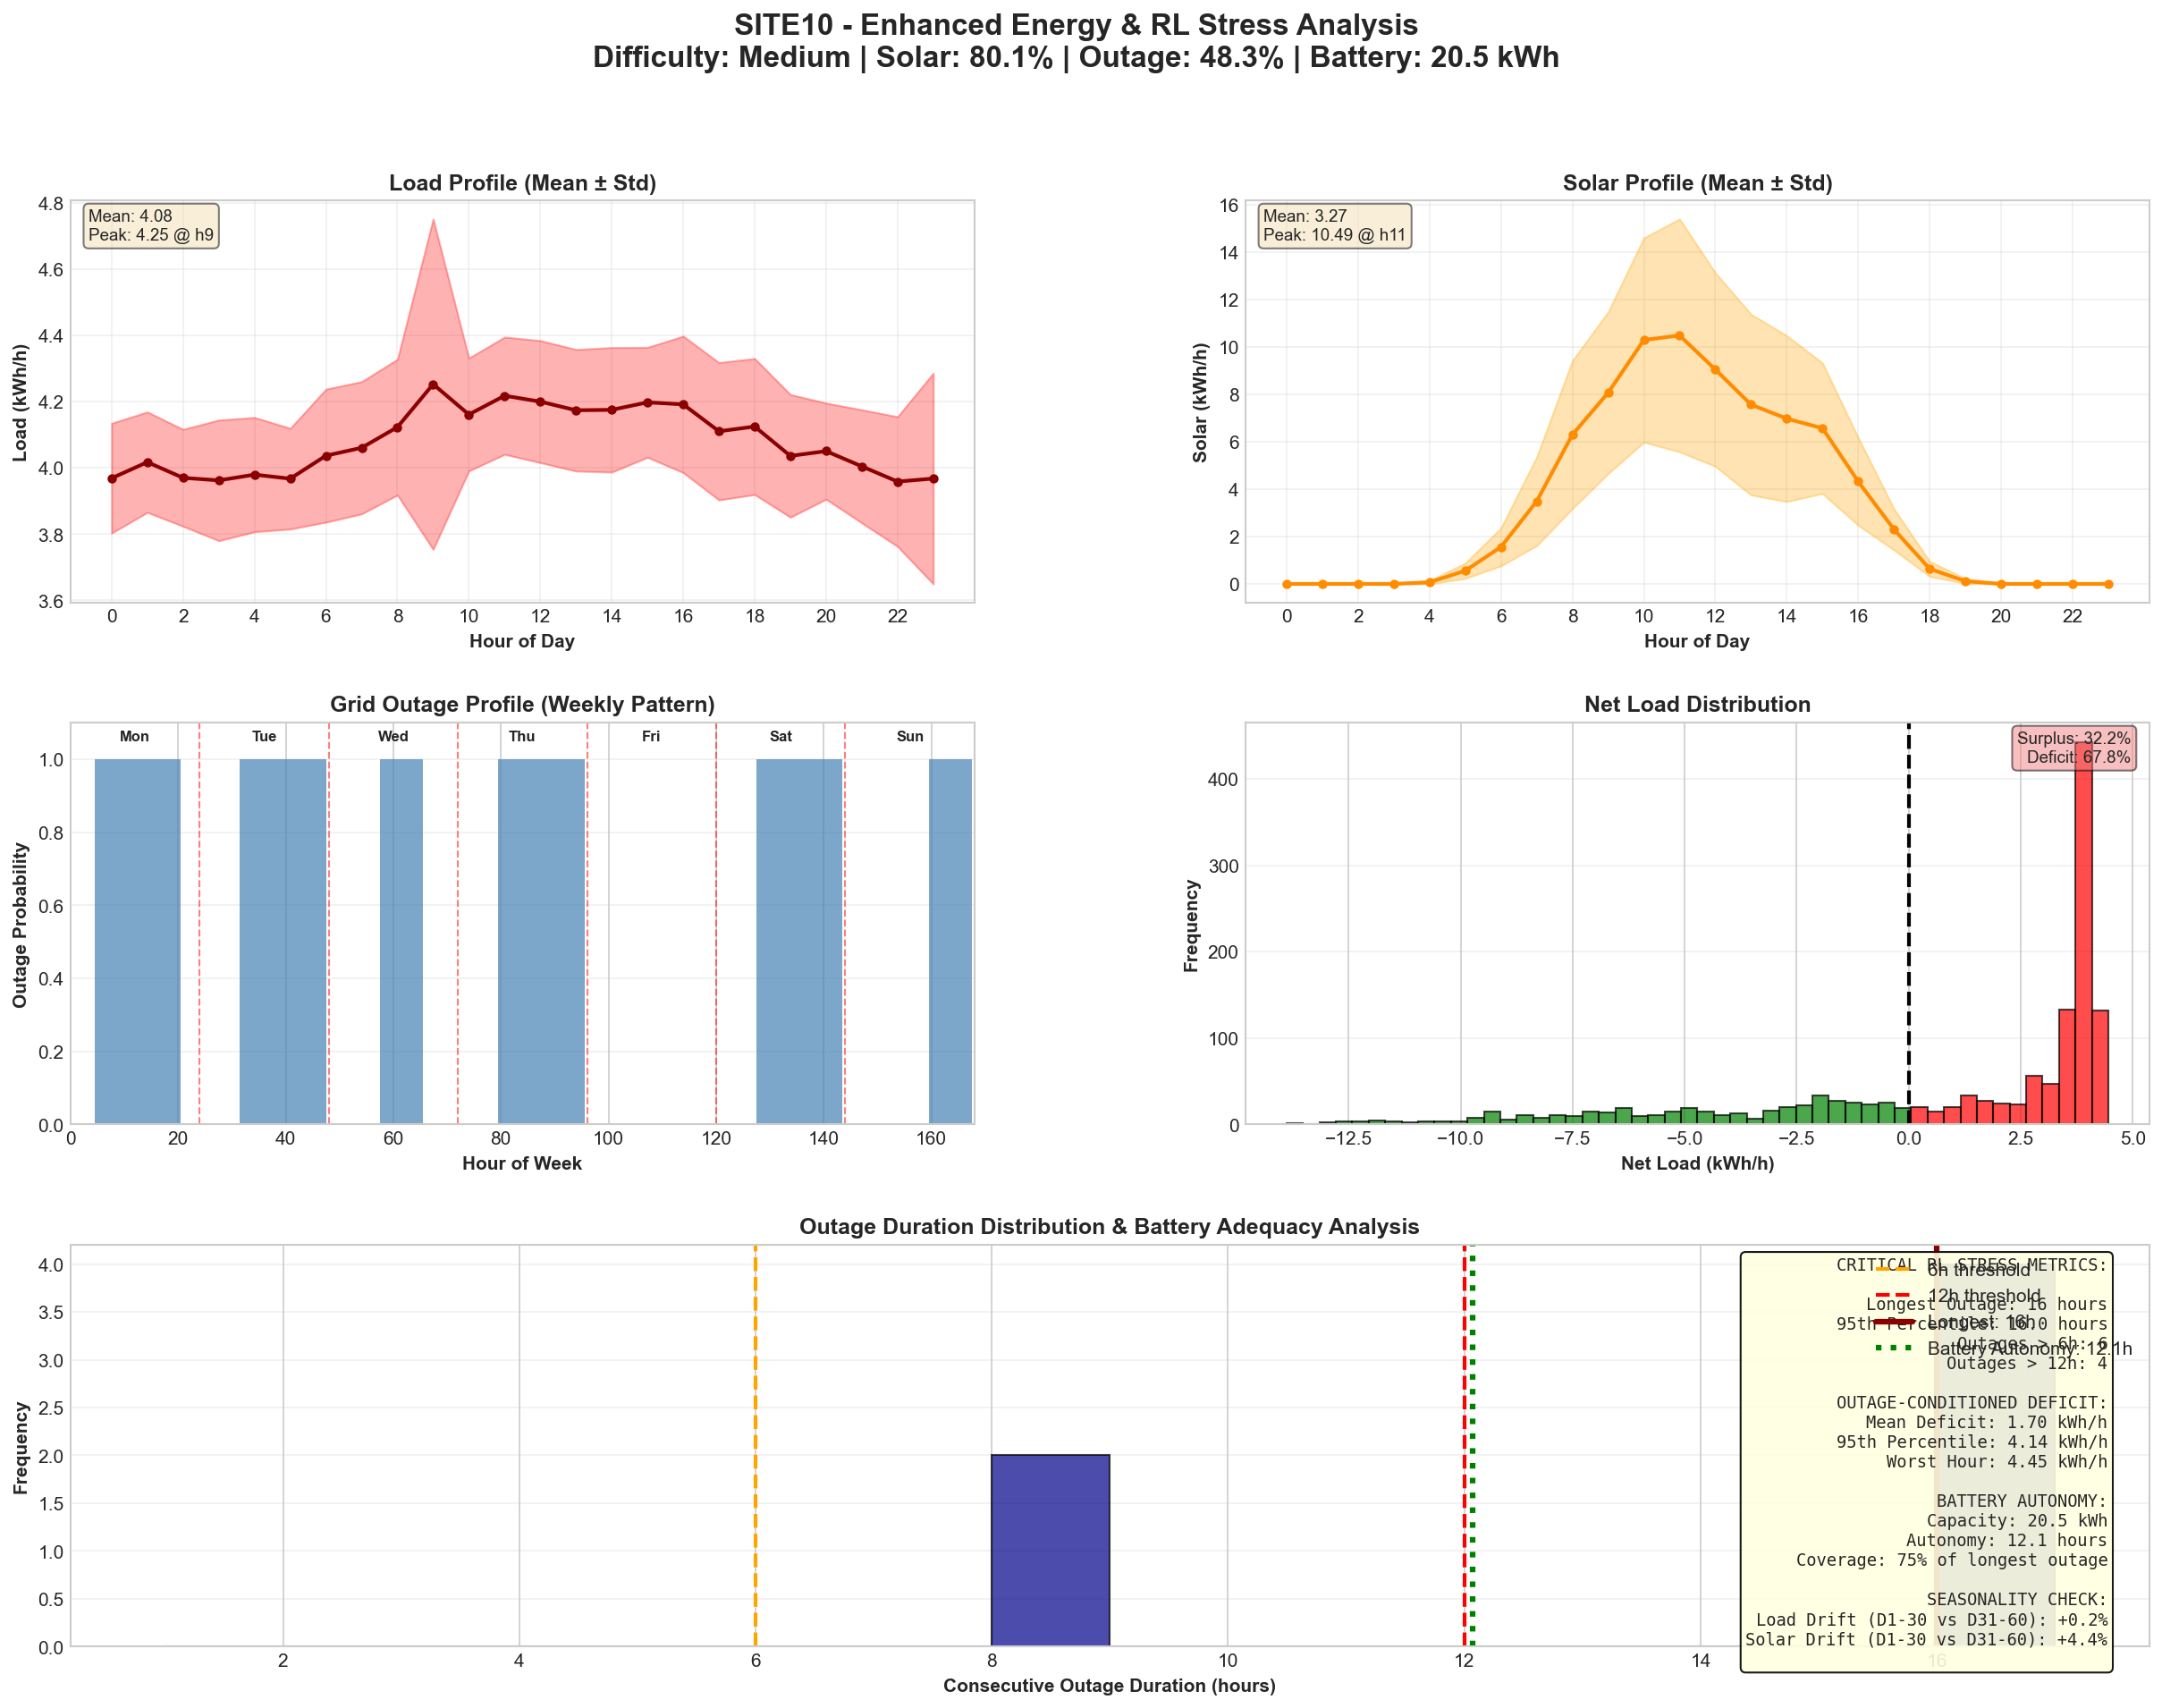
\includegraphics[width=\textwidth]{images/site10_enhanced_analysis}
\caption{Site~10 --- Medium (delayed-scenario edge case). Load mean
4.08\,kWh/h; solar coverage 80.1\%; battery autonomy 12.1\,h (75\% of
longest outage). Four outages exceed 12\,h. Despite a moderate composite score, high outage frequency (48.3\%)
combined with outages approaching battery autonomy makes this site
sensitive to logistics delays.}
\label{fig:app_site10}
\end{figure}
